\documentclass[notes,11pt, aspectratio=169]{beamer}
%based on https://github.com/paulgp/beamer-tips/blob/master/slides.tex

% \mode<presentation>
% {
%\usetheme{Pittsburgh} %a footerless theme
% \usetheme{Madrid}
% alternative, could always use
  %\usetheme{Rochester}
  %\usetheme{UGA}
  % \usefonttheme[onlysmall]{structurebold}
  % \useinnertheme[shadow=true]{rounded}
    % \usecolortheme{beaver} % This could be varied: UGA or cornell
  %\setbeamercolor{normal text}{fg=black}
  %\setbeamercolor{structure}{fg=black}
  % \setbeamercolor{structure}{bg=black}
  % \setbeamercolor{titlelike}{fg=black}

%
% Use this when we want notes
%
% }

\usepackage{pgfpages}
% These slides also contain speaker notes. You can print just the slides,
% just the notes, or both, depending on the setting below. Comment out the want
% you want.
\setbeameroption{hide notes} % Only slide
%\setbeameroption{show only notes} % Only notes
%\setbeameroption{show notes on second screen=right} % Both

\usepackage{helvet}
\usepackage[default]{lato}
\usepackage{array}

\setbeamertemplate{navigation symbols}{} %//removes the navigation symbols
\setbeamertemplate{frametitle continuation}[from second][\insertcontinuationcountroman]  %//to eliminate Roman numerals on 'first' slide when using allowframebreaks

%Bibliography options%
\usepackage[comma]{natbib}
\newcommand{\Cite}{\citet} % this for natbib
\bibpunct{(}{)}{;}{a}{}{;} %set if using natbib


\usepackage{tikz}
\usepackage{verbatim}
\setbeamertemplate{note page}{\pagecolor{yellow!5}\insertnote}
\setbeamertemplate{footline}[frame number]
\usetikzlibrary{positioning}
\usetikzlibrary{snakes}
\usetikzlibrary{calc}
\usetikzlibrary{arrows}
\usetikzlibrary{decorations.markings}
\usetikzlibrary{shapes.misc}
\usetikzlibrary{matrix,shapes,arrows,fit,tikzmark}
\usepackage{amsmath}
\usepackage{mathpazo}
\usepackage{hyperref}
\usepackage{lipsum}
\usepackage{multimedia}
\usepackage{graphicx}
\usepackage{multirow}
\usepackage{graphicx}
\usepackage{dcolumn}
\usepackage{bbm}
\newcolumntype{d}[0]{D{.}{.}{5}}


\usepackage{changepage}
\usepackage{appendixnumberbeamer}
\newcommand{\beginbackup}{
   \newcounter{framenumbervorappendix}
   \setcounter{framenumbervorappendix}{\value{framenumber}}
   \setbeamertemplate{footline}
   {
     \leavevmode%
     \hline
     box{%
       \begin{beamercolorbox}[wd=\paperwidth,ht=2.25ex,dp=1ex,right]{footlinecolor}%
%         \insertframenumber  \hspace*{2ex} 
       \end{beamercolorbox}}%
     \vskip0pt%
   }
 }
\newcommand{\backupend}{
   \addtocounter{framenumbervorappendix}{-\value{framenumber}}
   \addtocounter{framenumber}{\value{framenumbervorappendix}} 
}


\usepackage{graphicx}
\usepackage[space]{grffile}
\usepackage{booktabs}

% These are my colors -- there are many like them, but these ones are mine.
\definecolor{blue}{RGB}{0,114,178}
\definecolor{red}{RGB}{213,94,0}
\definecolor{yellow}{RGB}{240,228,66}
\definecolor{green}{RGB}{0,158,115}

\hypersetup{
  colorlinks=false,
  linkbordercolor = {white},
  linkcolor = {blue}
}


%% I use a beige off white for my background
\definecolor{MyBackground}{RGB}{255,253,218}

%% Uncomment this if you want to change the background color to something else
% \setbeamercolor{background canvas}{bg=MyBackground}
\setbeamercolor{background canvas}{bg=white}

%% Change the bg color to adjust your transition slide background color!
\newenvironment{transitionframe}{
  \setbeamercolor{background canvas}{bg=yellow}
  \begin{frame}}{
    \end{frame}
}

% \setbeamercolor{frametitle}{fg=blue}
% \setbeamercolor{title}{fg=black}
% \setbeamertemplate{footline}[frame number]
% \setbeamertemplate{navigation symbols}{} 
% \setbeamertemplate{itemize items}{-}
% \setbeamercolor{itemize item}{fg=blue}
% \setbeamercolor{itemize subitem}{fg=blue}
% \setbeamercolor{enumerate item}{fg=blue}
% \setbeamercolor{enumerate subitem}{fg=blue}
% \setbeamercolor{button}{bg=MyBackground,fg=blue,}



% If you like road maps, rather than having clutter at the top, have a roadmap show up at the end of each section 
% (and after your introduction)
% Uncomment this is if you want the roadmap!
% \AtBeginSection[]
% {
%    \begin{frame}
%        \frametitle{Roadmap of Talk}
%        \tableofcontents[currentsection]
%    \end{frame}
% }
\setbeamercolor{section in toc}{fg=blue}
\setbeamercolor{subsection in toc}{fg=red}
\setbeamersize{text margin left=1em,text margin right=1em} 

%-------------------- macros from TCILATEX.TEX --------------------------
% macros for user - defined functions
\def\limfunc#1{\mathop{\rm #1}}%
\def\func#1{\mathop{\rm #1}\nolimits}%
% macro for unit names
\def\unit#1{\mathop{\rm #1}\nolimits}%
% Macros for Scientific Word and Scientific WorkPlace 5.5 documents saved with the LaTeX filter.
% Copyright (C) 2005 Mackichan Software, Inc.

\typeout{TCILATEX Macros for Scientific Word and Scientific WorkPlace 5.5 <06 Oct 2005>.}
\typeout{NOTICE:  This macro file is NOT proprietary and may be 
freely copied and distributed.}
%
\makeatletter

%%%%%%%%%%%%%%%%%%%%%
% pdfTeX related.
\ifx\pdfoutput\relax\let\pdfoutput=\undefined\fi
\newcount\msipdfoutput
\ifx\pdfoutput\undefined
\else
 \ifcase\pdfoutput
 \else 
    \msipdfoutput=1
    \ifx\paperwidth\undefined
    \else
      \ifdim\paperheight=0pt\relax
      \else
        \pdfpageheight\paperheight
      \fi
      \ifdim\paperwidth=0pt\relax
      \else
        \pdfpagewidth\paperwidth
      \fi
    \fi
  \fi  
\fi

%%%%%%%%%%%%%%%%%%%%%
% FMTeXButton
% This is used for putting TeXButtons in the 
% frontmatter of a document. Add a line like
% \QTagDef{FMTeXButton}{101}{} to the filter 
% section of the cst being used. Also add a
% new section containing:
%     [f_101]
%     ALIAS=FMTexButton
%     TAG_TYPE=FIELD
%     TAG_LEADIN=TeX Button:
%
% It also works to put \defs in the preamble after 
% the \input tcilatex
\def\FMTeXButton#1{#1}
%
%%%%%%%%%%%%%%%%%%%%%%
% macros for time
\newcount\@hour\newcount\@minute\chardef\@x10\chardef\@xv60
\def\tcitime{
\def\@time{%
  \@minute\time\@hour\@minute\divide\@hour\@xv
  \ifnum\@hour<\@x 0\fi\the\@hour:%
  \multiply\@hour\@xv\advance\@minute-\@hour
  \ifnum\@minute<\@x 0\fi\the\@minute
  }}%

%%%%%%%%%%%%%%%%%%%%%%
% macro for hyperref and msihyperref
%\@ifundefined{hyperref}{\def\hyperref#1#2#3#4{#2\ref{#4}#3}}{}

\def\x@hyperref#1#2#3{%
   % Turn off various catcodes before reading parameter 4
   \catcode`\~ = 12
   \catcode`\$ = 12
   \catcode`\_ = 12
   \catcode`\# = 12
   \catcode`\& = 12
   \catcode`\% = 12
   \y@hyperref{#1}{#2}{#3}%
}

\def\y@hyperref#1#2#3#4{%
   #2\ref{#4}#3
   \catcode`\~ = 13
   \catcode`\$ = 3
   \catcode`\_ = 8
   \catcode`\# = 6
   \catcode`\& = 4
   \catcode`\% = 14
}

\@ifundefined{hyperref}{\let\hyperref\x@hyperref}{}
\@ifundefined{msihyperref}{\let\msihyperref\x@hyperref}{}




% macro for external program call
\@ifundefined{qExtProgCall}{\def\qExtProgCall#1#2#3#4#5#6{\relax}}{}
%%%%%%%%%%%%%%%%%%%%%%
%
% macros for graphics
%
\def\FILENAME#1{#1}%
%
\def\QCTOpt[#1]#2{%
  \def\QCTOptB{#1}
  \def\QCTOptA{#2}
}
\def\QCTNOpt#1{%
  \def\QCTOptA{#1}
  \let\QCTOptB\empty
}
\def\Qct{%
  \@ifnextchar[{%
    \QCTOpt}{\QCTNOpt}
}
\def\QCBOpt[#1]#2{%
  \def\QCBOptB{#1}%
  \def\QCBOptA{#2}%
}
\def\QCBNOpt#1{%
  \def\QCBOptA{#1}%
  \let\QCBOptB\empty
}
\def\Qcb{%
  \@ifnextchar[{%
    \QCBOpt}{\QCBNOpt}%
}
\def\PrepCapArgs{%
  \ifx\QCBOptA\empty
    \ifx\QCTOptA\empty
      {}%
    \else
      \ifx\QCTOptB\empty
        {\QCTOptA}%
      \else
        [\QCTOptB]{\QCTOptA}%
      \fi
    \fi
  \else
    \ifx\QCBOptA\empty
      {}%
    \else
      \ifx\QCBOptB\empty
        {\QCBOptA}%
      \else
        [\QCBOptB]{\QCBOptA}%
      \fi
    \fi
  \fi
}
\newcount\GRAPHICSTYPE
%\GRAPHICSTYPE 0 is for TurboTeX
%\GRAPHICSTYPE 1 is for DVIWindo (PostScript)
%%%(removed)%\GRAPHICSTYPE 2 is for psfig (PostScript)
\GRAPHICSTYPE=\z@
\def\GRAPHICSPS#1{%
 \ifcase\GRAPHICSTYPE%\GRAPHICSTYPE=0
   \special{ps: #1}%
 \or%\GRAPHICSTYPE=1
   \special{language "PS", include "#1"}%
%%%\or%\GRAPHICSTYPE=2
%%%  #1%
 \fi
}%
%
\def\GRAPHICSHP#1{\special{include #1}}%
%
% \graffile{ body }                                  %#1
%          { contentswidth (scalar)  }               %#2
%          { contentsheight (scalar) }               %#3
%          { vertical shift when in-line (scalar) }  %#4

\def\graffile#1#2#3#4{%
%%% \ifnum\GRAPHICSTYPE=\tw@
%%%  %Following if using psfig
%%%  \@ifundefined{psfig}{\input psfig.tex}{}%
%%%  \psfig{file=#1, height=#3, width=#2}%
%%% \else
  %Following for all others
  % JCS - added BOXTHEFRAME, see below
    \bgroup
	   \@inlabelfalse
       \leavevmode
       \@ifundefined{bbl@deactivate}{\def~{\string~}}{\activesoff}%
        \raise -#4 \BOXTHEFRAME{%
           \hbox to #2{\raise #3\hbox to #2{\null #1\hfil}}}%
    \egroup
}%
%
% A box for drafts
\def\draftbox#1#2#3#4{%
 \leavevmode\raise -#4 \hbox{%
  \frame{\rlap{\protect\tiny #1}\hbox to #2%
   {\vrule height#3 width\z@ depth\z@\hfil}%
  }%
 }%
}%
%
\newcount\@msidraft
\@msidraft=\z@
\let\nographics=\@msidraft
\newif\ifwasdraft
\wasdraftfalse

%  \GRAPHIC{ body }                                  %#1
%          { draft name }                            %#2
%          { contentswidth (scalar)  }               %#3
%          { contentsheight (scalar) }               %#4
%          { vertical shift when in-line (scalar) }  %#5
\def\GRAPHIC#1#2#3#4#5{%
   \ifnum\@msidraft=\@ne\draftbox{#2}{#3}{#4}{#5}%
   \else\graffile{#1}{#3}{#4}{#5}%
   \fi
}
%
\def\addtoLaTeXparams#1{%
    \edef\LaTeXparams{\LaTeXparams #1}}%
%
% JCS -  added a switch BoxFrame that can 
% be set by including X in the frame params.
% If set a box is drawn around the frame.

\newif\ifBoxFrame \BoxFramefalse
\newif\ifOverFrame \OverFramefalse
\newif\ifUnderFrame \UnderFramefalse

\def\BOXTHEFRAME#1{%
   \hbox{%
      \ifBoxFrame
         \frame{#1}%
      \else
         {#1}%
      \fi
   }%
}


\def\doFRAMEparams#1{\BoxFramefalse\OverFramefalse\UnderFramefalse\readFRAMEparams#1\end}%
\def\readFRAMEparams#1{%
 \ifx#1\end%
  \let\next=\relax
  \else
  \ifx#1i\dispkind=\z@\fi
  \ifx#1d\dispkind=\@ne\fi
  \ifx#1f\dispkind=\tw@\fi
  \ifx#1t\addtoLaTeXparams{t}\fi
  \ifx#1b\addtoLaTeXparams{b}\fi
  \ifx#1p\addtoLaTeXparams{p}\fi
  \ifx#1h\addtoLaTeXparams{h}\fi
  \ifx#1X\BoxFrametrue\fi
  \ifx#1O\OverFrametrue\fi
  \ifx#1U\UnderFrametrue\fi
  \ifx#1w
    \ifnum\@msidraft=1\wasdrafttrue\else\wasdraftfalse\fi
    \@msidraft=\@ne
  \fi
  \let\next=\readFRAMEparams
  \fi
 \next
 }%
%
%Macro for In-line graphics object
%   \IFRAME{ contentswidth (scalar)  }               %#1
%          { contentsheight (scalar) }               %#2
%          { vertical shift when in-line (scalar) }  %#3
%          { draft name }                            %#4
%          { body }                                  %#5
%          { caption}                                %#6


\def\IFRAME#1#2#3#4#5#6{%
      \bgroup
      \let\QCTOptA\empty
      \let\QCTOptB\empty
      \let\QCBOptA\empty
      \let\QCBOptB\empty
      #6%
      \parindent=0pt
      \leftskip=0pt
      \rightskip=0pt
      \setbox0=\hbox{\QCBOptA}%
      \@tempdima=#1\relax
      \ifOverFrame
          % Do this later
          \typeout{This is not implemented yet}%
          \show\HELP
      \else
         \ifdim\wd0>\@tempdima
            \advance\@tempdima by \@tempdima
            \ifdim\wd0 >\@tempdima
               \setbox1 =\vbox{%
                  \unskip\hbox to \@tempdima{\hfill\GRAPHIC{#5}{#4}{#1}{#2}{#3}\hfill}%
                  \unskip\hbox to \@tempdima{\parbox[b]{\@tempdima}{\QCBOptA}}%
               }%
               \wd1=\@tempdima
            \else
               \textwidth=\wd0
               \setbox1 =\vbox{%
                 \noindent\hbox to \wd0{\hfill\GRAPHIC{#5}{#4}{#1}{#2}{#3}\hfill}\\%
                 \noindent\hbox{\QCBOptA}%
               }%
               \wd1=\wd0
            \fi
         \else
            \ifdim\wd0>0pt
              \hsize=\@tempdima
              \setbox1=\vbox{%
                \unskip\GRAPHIC{#5}{#4}{#1}{#2}{0pt}%
                \break
                \unskip\hbox to \@tempdima{\hfill \QCBOptA\hfill}%
              }%
              \wd1=\@tempdima
           \else
              \hsize=\@tempdima
              \setbox1=\vbox{%
                \unskip\GRAPHIC{#5}{#4}{#1}{#2}{0pt}%
              }%
              \wd1=\@tempdima
           \fi
         \fi
         \@tempdimb=\ht1
         %\advance\@tempdimb by \dp1
         \advance\@tempdimb by -#2
         \advance\@tempdimb by #3
         \leavevmode
         \raise -\@tempdimb \hbox{\box1}%
      \fi
      \egroup%
}%
%
%Macro for Display graphics object
%   \DFRAME{ contentswidth (scalar)  }               %#1
%          { contentsheight (scalar) }               %#2
%          { draft label }                           %#3
%          { name }                                  %#4
%          { caption}                                %#5
\def\DFRAME#1#2#3#4#5{%
  \vspace\topsep
  \hfil\break
  \bgroup
     \leftskip\@flushglue
	 \rightskip\@flushglue
	 \parindent\z@
	 \parfillskip\z@skip
     \let\QCTOptA\empty
     \let\QCTOptB\empty
     \let\QCBOptA\empty
     \let\QCBOptB\empty
	 \vbox\bgroup
        \ifOverFrame 
           #5\QCTOptA\par
        \fi
        \GRAPHIC{#4}{#3}{#1}{#2}{\z@}%
        \ifUnderFrame 
           \break#5\QCBOptA
        \fi
	 \egroup
  \egroup
  \vspace\topsep
  \break
}%
%
%Macro for Floating graphic object
%   \FFRAME{ framedata f|i tbph x F|T }              %#1
%          { contentswidth (scalar)  }               %#2
%          { contentsheight (scalar) }               %#3
%          { caption }                               %#4
%          { label }                                 %#5
%          { draft name }                            %#6
%          { body }                                  %#7
\def\FFRAME#1#2#3#4#5#6#7{%
 %If float.sty loaded and float option is 'h', change to 'H'  (gp) 1998/09/05
  \@ifundefined{floatstyle}
    {%floatstyle undefined (and float.sty not present), no change
     \begin{figure}[#1]%
    }
    {%floatstyle DEFINED
	 \ifx#1h%Only the h parameter, change to H
      \begin{figure}[H]%
	 \else
      \begin{figure}[#1]%
	 \fi
	}
  \let\QCTOptA\empty
  \let\QCTOptB\empty
  \let\QCBOptA\empty
  \let\QCBOptB\empty
  \ifOverFrame
    #4
    \ifx\QCTOptA\empty
    \else
      \ifx\QCTOptB\empty
        \caption{\QCTOptA}%
      \else
        \caption[\QCTOptB]{\QCTOptA}%
      \fi
    \fi
    \ifUnderFrame\else
      \label{#5}%
    \fi
  \else
    \UnderFrametrue%
  \fi
  \begin{center}\GRAPHIC{#7}{#6}{#2}{#3}{\z@}\end{center}%
  \ifUnderFrame
    #4
    \ifx\QCBOptA\empty
      \caption{}%
    \else
      \ifx\QCBOptB\empty
        \caption{\QCBOptA}%
      \else
        \caption[\QCBOptB]{\QCBOptA}%
      \fi
    \fi
    \label{#5}%
  \fi
  \end{figure}%
 }%
%
%
%    \FRAME{ framedata f|i tbph x F|T }              %#1
%          { contentswidth (scalar)  }               %#2
%          { contentsheight (scalar) }               %#3
%          { vertical shift when in-line (scalar) }  %#4
%          { caption }                               %#5
%          { label }                                 %#6
%          { name }                                  %#7
%          { body }                                  %#8
%
%    framedata is a string which can contain the following
%    characters: idftbphxFT
%    Their meaning is as follows:
%             i, d or f : in-line, display, or floating
%             t,b,p,h   : LaTeX floating placement options
%             x         : fit contents box to contents
%             F or T    : Figure or Table. 
%                         Later this can expand
%                         to a more general float class.
%
%
\newcount\dispkind%

\def\makeactives{
  \catcode`\"=\active
  \catcode`\;=\active
  \catcode`\:=\active
  \catcode`\'=\active
  \catcode`\~=\active
}
\bgroup
   \makeactives
   \gdef\activesoff{%
      \def"{\string"}%
      \def;{\string;}%
      \def:{\string:}%
      \def'{\string'}%
      \def~{\string~}%
      %\bbl@deactivate{"}%
      %\bbl@deactivate{;}%
      %\bbl@deactivate{:}%
      %\bbl@deactivate{'}%
    }
\egroup

\def\FRAME#1#2#3#4#5#6#7#8{%
 \bgroup
 \ifnum\@msidraft=\@ne
   \wasdrafttrue
 \else
   \wasdraftfalse%
 \fi
 \def\LaTeXparams{}%
 \dispkind=\z@
 \def\LaTeXparams{}%
 \doFRAMEparams{#1}%
 \ifnum\dispkind=\z@\IFRAME{#2}{#3}{#4}{#7}{#8}{#5}\else
  \ifnum\dispkind=\@ne\DFRAME{#2}{#3}{#7}{#8}{#5}\else
   \ifnum\dispkind=\tw@
    \edef\@tempa{\noexpand\FFRAME{\LaTeXparams}}%
    \@tempa{#2}{#3}{#5}{#6}{#7}{#8}%
    \fi
   \fi
  \fi
  \ifwasdraft\@msidraft=1\else\@msidraft=0\fi{}%
  \egroup
 }%
%
% This macro added to let SW gobble a parameter that
% should not be passed on and expanded. 

\def\TEXUX#1{"texux"}

%
% Macros for text attributes:
%
\def\BF#1{{\bf {#1}}}%
\def\NEG#1{\leavevmode\hbox{\rlap{\thinspace/}{$#1$}}}%
%
%%%%%%%%%%%%%%%%%%%%%%%%%%%%%%%%%%%%%%%%%%%%%%%%%%%%%%%%%%%%%%%%%%%%%%%%
%
%
% macros for user - defined functions
\def\limfunc#1{\mathop{\rm #1}}%
\def\func#1{\mathop{\rm #1}\nolimits}%
% macro for unit names
\def\unit#1{\mathord{\thinspace\rm #1}}%

%
% miscellaneous 
\long\def\QQQ#1#2{%
     \long\expandafter\def\csname#1\endcsname{#2}}%
\@ifundefined{QTP}{\def\QTP#1{}}{}
\@ifundefined{QEXCLUDE}{\def\QEXCLUDE#1{}}{}
\@ifundefined{Qlb}{\def\Qlb#1{#1}}{}
\@ifundefined{Qlt}{\def\Qlt#1{#1}}{}
\def\QWE{}%
\long\def\QQA#1#2{}%
\def\QTR#1#2{{\csname#1\endcsname {#2}}}%
  %	Add aliases for the ulem package
  \let\QQQuline\uline
  \let\QQQsout\sout
  \let\QQQuuline\uuline
  \let\QQQuwave\uwave
  \let\QQQxout\xout
\long\def\TeXButton#1#2{#2}%
\long\def\QSubDoc#1#2{#2}%
\def\EXPAND#1[#2]#3{}%
\def\NOEXPAND#1[#2]#3{}%
\def\PROTECTED{}%
\def\LaTeXparent#1{}%
\def\ChildStyles#1{}%
\def\ChildDefaults#1{}%
\def\QTagDef#1#2#3{}%

% Constructs added with Scientific Notebook
\@ifundefined{correctchoice}{\def\correctchoice{\relax}}{}
\@ifundefined{HTML}{\def\HTML#1{\relax}}{}
\@ifundefined{TCIIcon}{\def\TCIIcon#1#2#3#4{\relax}}{}
\if@compatibility
  \typeout{Not defining UNICODE  U or CustomNote commands for LaTeX 2.09.}
\else
  \providecommand{\UNICODE}[2][]{\protect\rule{.1in}{.1in}}
  \providecommand{\U}[1]{\protect\rule{.1in}{.1in}}
  \providecommand{\CustomNote}[3][]{\marginpar{#3}}
\fi

\@ifundefined{lambdabar}{
      \def\lambdabar{\errmessage{You have used the lambdabar symbol. 
                      This is available for typesetting only in RevTeX styles.}}
   }{}

%
% Macros for style editor docs
\@ifundefined{StyleEditBeginDoc}{\def\StyleEditBeginDoc{\relax}}{}
%
% Macros for footnotes
\def\QQfnmark#1{\footnotemark}
\def\QQfntext#1#2{\addtocounter{footnote}{#1}\footnotetext{#2}}
%
% Macros for indexing.
%
\@ifundefined{TCIMAKEINDEX}{}{\makeindex}%
%
% Attempts to avoid problems with other styles
\@ifundefined{abstract}{%
 \def\abstract{%
  \if@twocolumn
   \section*{Abstract (Not appropriate in this style!)}%
   \else \small 
   \begin{center}{\bf Abstract\vspace{-.5em}\vspace{\z@}}\end{center}%
   \quotation 
   \fi
  }%
 }{%
 }%
\@ifundefined{endabstract}{\def\endabstract
  {\if@twocolumn\else\endquotation\fi}}{}%
\@ifundefined{maketitle}{\def\maketitle#1{}}{}%
\@ifundefined{affiliation}{\def\affiliation#1{}}{}%
\@ifundefined{proof}{\def\proof{\noindent{\bfseries Proof. }}}{}%
\@ifundefined{endproof}{\def\endproof{\mbox{\ \rule{.1in}{.1in}}}}{}%
\@ifundefined{newfield}{\def\newfield#1#2{}}{}%
\@ifundefined{chapter}{\def\chapter#1{\par(Chapter head:)#1\par }%
 \newcount\c@chapter}{}%
\@ifundefined{part}{\def\part#1{\par(Part head:)#1\par }}{}%
\@ifundefined{section}{\def\section#1{\par(Section head:)#1\par }}{}%
\@ifundefined{subsection}{\def\subsection#1%
 {\par(Subsection head:)#1\par }}{}%
\@ifundefined{subsubsection}{\def\subsubsection#1%
 {\par(Subsubsection head:)#1\par }}{}%
\@ifundefined{paragraph}{\def\paragraph#1%
 {\par(Subsubsubsection head:)#1\par }}{}%
\@ifundefined{subparagraph}{\def\subparagraph#1%
 {\par(Subsubsubsubsection head:)#1\par }}{}%
%%%%%%%%%%%%%%%%%%%%%%%%%%%%%%%%%%%%%%%%%%%%%%%%%%%%%%%%%%%%%%%%%%%%%%%%
% These symbols are not recognized by LaTeX
\@ifundefined{therefore}{\def\therefore{}}{}%
\@ifundefined{backepsilon}{\def\backepsilon{}}{}%
\@ifundefined{yen}{\def\yen{\hbox{\rm\rlap=Y}}}{}%
\@ifundefined{registered}{%
   \def\registered{\relax\ifmmode{}\r@gistered
                    \else$\m@th\r@gistered$\fi}%
 \def\r@gistered{^{\ooalign
  {\hfil\raise.07ex\hbox{$\scriptstyle\rm\text{R}$}\hfil\crcr
  \mathhexbox20D}}}}{}%
\@ifundefined{Eth}{\def\Eth{}}{}%
\@ifundefined{eth}{\def\eth{}}{}%
\@ifundefined{Thorn}{\def\Thorn{}}{}%
\@ifundefined{thorn}{\def\thorn{}}{}%
% A macro to allow any symbol that requires math to appear in text
\def\TEXTsymbol#1{\mbox{$#1$}}%
\@ifundefined{degree}{\def\degree{{}^{\circ}}}{}%
%
% macros for T3TeX files
\newdimen\theight
\@ifundefined{Column}{\def\Column{%
 \vadjust{\setbox\z@=\hbox{\scriptsize\quad\quad tcol}%
  \theight=\ht\z@\advance\theight by \dp\z@\advance\theight by \lineskip
  \kern -\theight \vbox to \theight{%
   \rightline{\rlap{\box\z@}}%
   \vss
   }%
  }%
 }}{}%
%
\@ifundefined{qed}{\def\qed{%
 \ifhmode\unskip\nobreak\fi\ifmmode\ifinner\else\hskip5\p@\fi\fi
 \hbox{\hskip5\p@\vrule width4\p@ height6\p@ depth1.5\p@\hskip\p@}%
 }}{}%
%
\@ifundefined{cents}{\def\cents{\hbox{\rm\rlap c/}}}{}%
\@ifundefined{tciLaplace}{\def\tciLaplace{\ensuremath{\mathcal{L}}}}{}%
\@ifundefined{tciFourier}{\def\tciFourier{\ensuremath{\mathcal{F}}}}{}%
\@ifundefined{textcurrency}{\def\textcurrency{\hbox{\rm\rlap xo}}}{}%
\@ifundefined{texteuro}{\def\texteuro{\hbox{\rm\rlap C=}}}{}%
\@ifundefined{euro}{\def\euro{\hbox{\rm\rlap C=}}}{}%
\@ifundefined{textfranc}{\def\textfranc{\hbox{\rm\rlap-F}}}{}%
\@ifundefined{textlira}{\def\textlira{\hbox{\rm\rlap L=}}}{}%
\@ifundefined{textpeseta}{\def\textpeseta{\hbox{\rm P\negthinspace s}}}{}%
%
\@ifundefined{miss}{\def\miss{\hbox{\vrule height2\p@ width 2\p@ depth\z@}}}{}%
%
\@ifundefined{vvert}{\def\vvert{\Vert}}{}%  %always translated to \left| or \right|
%
\@ifundefined{tcol}{\def\tcol#1{{\baselineskip=6\p@ \vcenter{#1}} \Column}}{}%
%
\@ifundefined{dB}{\def\dB{\hbox{{}}}}{}%        %dummy entry in column 
\@ifundefined{mB}{\def\mB#1{\hbox{$#1$}}}{}%   %column entry
\@ifundefined{nB}{\def\nB#1{\hbox{#1}}}{}%     %column entry (not math)
%
\@ifundefined{note}{\def\note{$^{\dag}}}{}%
%
\def\newfmtname{LaTeX2e}
% No longer load latexsym.  This is now handled by SWP, which uses amsfonts if necessary
%
\ifx\fmtname\newfmtname
  \DeclareOldFontCommand{\rm}{\normalfont\rmfamily}{\mathrm}
  \DeclareOldFontCommand{\sf}{\normalfont\sffamily}{\mathsf}
  \DeclareOldFontCommand{\tt}{\normalfont\ttfamily}{\mathtt}
  \DeclareOldFontCommand{\bf}{\normalfont\bfseries}{\mathbf}
  \DeclareOldFontCommand{\it}{\normalfont\itshape}{\mathit}
  \DeclareOldFontCommand{\sl}{\normalfont\slshape}{\@nomath\sl}
  \DeclareOldFontCommand{\sc}{\normalfont\scshape}{\@nomath\sc}
\fi

%
% Greek bold macros
% Redefine all of the math symbols 
% which might be bolded	 - there are 
% probably others to add to this list

\def\alpha{{\Greekmath 010B}}%
\def\beta{{\Greekmath 010C}}%
\def\gamma{{\Greekmath 010D}}%
\def\delta{{\Greekmath 010E}}%
\def\epsilon{{\Greekmath 010F}}%
\def\zeta{{\Greekmath 0110}}%
\def\eta{{\Greekmath 0111}}%
\def\theta{{\Greekmath 0112}}%
\def\iota{{\Greekmath 0113}}%
\def\kappa{{\Greekmath 0114}}%
\def\lambda{{\Greekmath 0115}}%
\def\mu{{\Greekmath 0116}}%
\def\nu{{\Greekmath 0117}}%
\def\xi{{\Greekmath 0118}}%
\def\pi{{\Greekmath 0119}}%
\def\rho{{\Greekmath 011A}}%
\def\sigma{{\Greekmath 011B}}%
\def\tau{{\Greekmath 011C}}%
\def\upsilon{{\Greekmath 011D}}%
\def\phi{{\Greekmath 011E}}%
\def\chi{{\Greekmath 011F}}%
\def\psi{{\Greekmath 0120}}%
\def\omega{{\Greekmath 0121}}%
\def\varepsilon{{\Greekmath 0122}}%
\def\vartheta{{\Greekmath 0123}}%
\def\varpi{{\Greekmath 0124}}%
\def\varrho{{\Greekmath 0125}}%
\def\varsigma{{\Greekmath 0126}}%
\def\varphi{{\Greekmath 0127}}%

\def\nabla{{\Greekmath 0272}}
\def\FindBoldGroup{%
   {\setbox0=\hbox{$\mathbf{x\global\edef\theboldgroup{\the\mathgroup}}$}}%
}

\def\Greekmath#1#2#3#4{%
    \if@compatibility
        \ifnum\mathgroup=\symbold
           \mathchoice{\mbox{\boldmath$\displaystyle\mathchar"#1#2#3#4$}}%
                      {\mbox{\boldmath$\textstyle\mathchar"#1#2#3#4$}}%
                      {\mbox{\boldmath$\scriptstyle\mathchar"#1#2#3#4$}}%
                      {\mbox{\boldmath$\scriptscriptstyle\mathchar"#1#2#3#4$}}%
        \else
           \mathchar"#1#2#3#4% 
        \fi 
    \else 
        \FindBoldGroup
        \ifnum\mathgroup=\theboldgroup % For 2e
           \mathchoice{\mbox{\boldmath$\displaystyle\mathchar"#1#2#3#4$}}%
                      {\mbox{\boldmath$\textstyle\mathchar"#1#2#3#4$}}%
                      {\mbox{\boldmath$\scriptstyle\mathchar"#1#2#3#4$}}%
                      {\mbox{\boldmath$\scriptscriptstyle\mathchar"#1#2#3#4$}}%
        \else
           \mathchar"#1#2#3#4% 
        \fi     	    
	  \fi}

\newif\ifGreekBold  \GreekBoldfalse
\let\SAVEPBF=\pbf
\def\pbf{\GreekBoldtrue\SAVEPBF}%
%

\@ifundefined{theorem}{\newtheorem{theorem}{Theorem}}{}
\@ifundefined{lemma}{\newtheorem{lemma}[theorem]{Lemma}}{}
\@ifundefined{corollary}{\newtheorem{corollary}[theorem]{Corollary}}{}
\@ifundefined{conjecture}{\newtheorem{conjecture}[theorem]{Conjecture}}{}
\@ifundefined{proposition}{\newtheorem{proposition}[theorem]{Proposition}}{}
\@ifundefined{axiom}{\newtheorem{axiom}{Axiom}}{}
\@ifundefined{remark}{\newtheorem{remark}{Remark}}{}
\@ifundefined{example}{\newtheorem{example}{Example}}{}
\@ifundefined{exercise}{\newtheorem{exercise}{Exercise}}{}
\@ifundefined{definition}{\newtheorem{definition}{Definition}}{}


\@ifundefined{mathletters}{%
  %\def\theequation{\arabic{equation}}
  \newcounter{equationnumber}  
  \def\mathletters{%
     \addtocounter{equation}{1}
     \edef\@currentlabel{\theequation}%
     \setcounter{equationnumber}{\c@equation}
     \setcounter{equation}{0}%
     \edef\theequation{\@currentlabel\noexpand\alph{equation}}%
  }
  \def\endmathletters{%
     \setcounter{equation}{\value{equationnumber}}%
  }
}{}

%Logos
\@ifundefined{BibTeX}{%
    \def\BibTeX{{\rm B\kern-.05em{\sc i\kern-.025em b}\kern-.08em
                 T\kern-.1667em\lower.7ex\hbox{E}\kern-.125emX}}}{}%
\@ifundefined{AmS}%
    {\def\AmS{{\protect\usefont{OMS}{cmsy}{m}{n}%
                A\kern-.1667em\lower.5ex\hbox{M}\kern-.125emS}}}{}%
\@ifundefined{AmSTeX}{\def\AmSTeX{\protect\AmS-\protect\TeX\@}}{}%
%

% This macro is a fix to eqnarray
\def\@@eqncr{\let\@tempa\relax
    \ifcase\@eqcnt \def\@tempa{& & &}\or \def\@tempa{& &}%
      \else \def\@tempa{&}\fi
     \@tempa
     \if@eqnsw
        \iftag@
           \@taggnum
        \else
           \@eqnnum\stepcounter{equation}%
        \fi
     \fi
     \global\tag@false
     \global\@eqnswtrue
     \global\@eqcnt\z@\cr}


\def\TCItag{\@ifnextchar*{\@TCItagstar}{\@TCItag}}
\def\@TCItag#1{%
    \global\tag@true
    \global\def\@taggnum{(#1)}%
    \global\def\@currentlabel{#1}}
\def\@TCItagstar*#1{%
    \global\tag@true
    \global\def\@taggnum{#1}%
    \global\def\@currentlabel{#1}}
%
%%%%%%%%%%%%%%%%%%%%%%%%%%%%%%%%%%%%%%%%%%%%%%%%%%%%%%%%%%%%%%%%%%%%%
%
\def\QATOP#1#2{{#1 \atop #2}}%
\def\QTATOP#1#2{{\textstyle {#1 \atop #2}}}%
\def\QDATOP#1#2{{\displaystyle {#1 \atop #2}}}%
\def\QABOVE#1#2#3{{#2 \above#1 #3}}%
\def\QTABOVE#1#2#3{{\textstyle {#2 \above#1 #3}}}%
\def\QDABOVE#1#2#3{{\displaystyle {#2 \above#1 #3}}}%
\def\QOVERD#1#2#3#4{{#3 \overwithdelims#1#2 #4}}%
\def\QTOVERD#1#2#3#4{{\textstyle {#3 \overwithdelims#1#2 #4}}}%
\def\QDOVERD#1#2#3#4{{\displaystyle {#3 \overwithdelims#1#2 #4}}}%
\def\QATOPD#1#2#3#4{{#3 \atopwithdelims#1#2 #4}}%
\def\QTATOPD#1#2#3#4{{\textstyle {#3 \atopwithdelims#1#2 #4}}}%
\def\QDATOPD#1#2#3#4{{\displaystyle {#3 \atopwithdelims#1#2 #4}}}%
\def\QABOVED#1#2#3#4#5{{#4 \abovewithdelims#1#2#3 #5}}%
\def\QTABOVED#1#2#3#4#5{{\textstyle 
   {#4 \abovewithdelims#1#2#3 #5}}}%
\def\QDABOVED#1#2#3#4#5{{\displaystyle 
   {#4 \abovewithdelims#1#2#3 #5}}}%
%
% Macros for text size operators:
%

\def\tint{\msi@int\textstyle\int}%
\def\tiint{\msi@int\textstyle\iint}%
\def\tiiint{\msi@int\textstyle\iiint}%
\def\tiiiint{\msi@int\textstyle\iiiint}%
\def\tidotsint{\msi@int\textstyle\idotsint}%
\def\toint{\msi@int\textstyle\oint}%


\def\tsum{\mathop{\textstyle \sum }}%
\def\tprod{\mathop{\textstyle \prod }}%
\def\tbigcap{\mathop{\textstyle \bigcap }}%
\def\tbigwedge{\mathop{\textstyle \bigwedge }}%
\def\tbigoplus{\mathop{\textstyle \bigoplus }}%
\def\tbigodot{\mathop{\textstyle \bigodot }}%
\def\tbigsqcup{\mathop{\textstyle \bigsqcup }}%
\def\tcoprod{\mathop{\textstyle \coprod }}%
\def\tbigcup{\mathop{\textstyle \bigcup }}%
\def\tbigvee{\mathop{\textstyle \bigvee }}%
\def\tbigotimes{\mathop{\textstyle \bigotimes }}%
\def\tbiguplus{\mathop{\textstyle \biguplus }}%
%
%
%Macros for display size operators:
%

\newtoks\temptoksa
\newtoks\temptoksb
\newtoks\temptoksc


\def\msi@int#1#2{%
 \def\@temp{{#1#2\the\temptoksc_{\the\temptoksa}^{\the\temptoksb}}}%   
 \futurelet\@nextcs
 \@int
}

\def\@int{%
   \ifx\@nextcs\limits
      \typeout{Found limits}%
      \temptoksc={\limits}%
	  \let\@next\@intgobble%
   \else\ifx\@nextcs\nolimits
      \typeout{Found nolimits}%
      \temptoksc={\nolimits}%
	  \let\@next\@intgobble%
   \else
      \typeout{Did not find limits or no limits}%
      \temptoksc={}%
      \let\@next\msi@limits%
   \fi\fi
   \@next   
}%

\def\@intgobble#1{%
   \typeout{arg is #1}%
   \msi@limits
}


\def\msi@limits{%
   \temptoksa={}%
   \temptoksb={}%
   \@ifnextchar_{\@limitsa}{\@limitsb}%
}

\def\@limitsa_#1{%
   \temptoksa={#1}%
   \@ifnextchar^{\@limitsc}{\@temp}%
}

\def\@limitsb{%
   \@ifnextchar^{\@limitsc}{\@temp}%
}

\def\@limitsc^#1{%
   \temptoksb={#1}%
   \@ifnextchar_{\@limitsd}{\@temp}%   
}

\def\@limitsd_#1{%
   \temptoksa={#1}%
   \@temp
}



\def\dint{\msi@int\displaystyle\int}%
\def\diint{\msi@int\displaystyle\iint}%
\def\diiint{\msi@int\displaystyle\iiint}%
\def\diiiint{\msi@int\displaystyle\iiiint}%
\def\didotsint{\msi@int\displaystyle\idotsint}%
\def\doint{\msi@int\displaystyle\oint}%

\def\dsum{\mathop{\displaystyle \sum }}%
\def\dprod{\mathop{\displaystyle \prod }}%
\def\dbigcap{\mathop{\displaystyle \bigcap }}%
\def\dbigwedge{\mathop{\displaystyle \bigwedge }}%
\def\dbigoplus{\mathop{\displaystyle \bigoplus }}%
\def\dbigodot{\mathop{\displaystyle \bigodot }}%
\def\dbigsqcup{\mathop{\displaystyle \bigsqcup }}%
\def\dcoprod{\mathop{\displaystyle \coprod }}%
\def\dbigcup{\mathop{\displaystyle \bigcup }}%
\def\dbigvee{\mathop{\displaystyle \bigvee }}%
\def\dbigotimes{\mathop{\displaystyle \bigotimes }}%
\def\dbiguplus{\mathop{\displaystyle \biguplus }}%

\if@compatibility\else
  % Always load amsmath in LaTeX2e mode
  \RequirePackage{amsmath}
\fi

\def\ExitTCILatex{\makeatother\endinput}

\bgroup
\ifx\ds@amstex\relax
   \message{amstex already loaded}\aftergroup\ExitTCILatex
\else
   \@ifpackageloaded{amsmath}%
      {\if@compatibility\message{amsmath already loaded}\fi\aftergroup\ExitTCILatex}
      {}
   \@ifpackageloaded{amstex}%
      {\if@compatibility\message{amstex already loaded}\fi\aftergroup\ExitTCILatex}
      {}
   \@ifpackageloaded{amsgen}%
      {\if@compatibility\message{amsgen already loaded}\fi\aftergroup\ExitTCILatex}
      {}
\fi
\egroup

%Exit if any of the AMS macros are already loaded.
%This is always the case for LaTeX2e mode.


%%%%%%%%%%%%%%%%%%%%%%%%%%%%%%%%%%%%%%%%%%%%%%%%%%%%%%%%%%%%%%%%%%%%%%%%%%
% NOTE: The rest of this file is read only if in LaTeX 2.09 compatibility
% mode. This section is used to define AMS-like constructs in the
% event they have not been defined.
%%%%%%%%%%%%%%%%%%%%%%%%%%%%%%%%%%%%%%%%%%%%%%%%%%%%%%%%%%%%%%%%%%%%%%%%%%
\typeout{TCILATEX defining AMS-like constructs in LaTeX 2.09 COMPATIBILITY MODE}
%%%%%%%%%%%%%%%%%%%%%%%%%%%%%%%%%%%%%%%%%%%%%%%%%%%%%%%%%%%%%%%%%%%%%%%%
%  Macros to define some AMS LaTeX constructs when 
%  AMS LaTeX has not been loaded
% 
% These macros are copied from the AMS-TeX package for doing
% multiple integrals.
%
\let\DOTSI\relax
\def\RIfM@{\relax\ifmmode}%
\def\FN@{\futurelet\next}%
\newcount\intno@
\def\iint{\DOTSI\intno@\tw@\FN@\ints@}%
\def\iiint{\DOTSI\intno@\thr@@\FN@\ints@}%
\def\iiiint{\DOTSI\intno@4 \FN@\ints@}%
\def\idotsint{\DOTSI\intno@\z@\FN@\ints@}%
\def\ints@{\findlimits@\ints@@}%
\newif\iflimtoken@
\newif\iflimits@
\def\findlimits@{\limtoken@true\ifx\next\limits\limits@true
 \else\ifx\next\nolimits\limits@false\else
 \limtoken@false\ifx\ilimits@\nolimits\limits@false\else
 \ifinner\limits@false\else\limits@true\fi\fi\fi\fi}%
\def\multint@{\int\ifnum\intno@=\z@\intdots@                          %1
 \else\intkern@\fi                                                    %2
 \ifnum\intno@>\tw@\int\intkern@\fi                                   %3
 \ifnum\intno@>\thr@@\int\intkern@\fi                                 %4
 \int}%                                                               %5
\def\multintlimits@{\intop\ifnum\intno@=\z@\intdots@\else\intkern@\fi
 \ifnum\intno@>\tw@\intop\intkern@\fi
 \ifnum\intno@>\thr@@\intop\intkern@\fi\intop}%
\def\intic@{%
    \mathchoice{\hskip.5em}{\hskip.4em}{\hskip.4em}{\hskip.4em}}%
\def\negintic@{\mathchoice
 {\hskip-.5em}{\hskip-.4em}{\hskip-.4em}{\hskip-.4em}}%
\def\ints@@{\iflimtoken@                                              %1
 \def\ints@@@{\iflimits@\negintic@
   \mathop{\intic@\multintlimits@}\limits                             %2
  \else\multint@\nolimits\fi                                          %3
  \eat@}%                                                             %4
 \else                                                                %5
 \def\ints@@@{\iflimits@\negintic@
  \mathop{\intic@\multintlimits@}\limits\else
  \multint@\nolimits\fi}\fi\ints@@@}%
\def\intkern@{\mathchoice{\!\!\!}{\!\!}{\!\!}{\!\!}}%
\def\plaincdots@{\mathinner{\cdotp\cdotp\cdotp}}%
\def\intdots@{\mathchoice{\plaincdots@}%
 {{\cdotp}\mkern1.5mu{\cdotp}\mkern1.5mu{\cdotp}}%
 {{\cdotp}\mkern1mu{\cdotp}\mkern1mu{\cdotp}}%
 {{\cdotp}\mkern1mu{\cdotp}\mkern1mu{\cdotp}}}%
%
%
%  These macros are for doing the AMS \text{} construct
%
\def\RIfM@{\relax\protect\ifmmode}
\def\text{\RIfM@\expandafter\text@\else\expandafter\mbox\fi}
\let\nfss@text\text
\def\text@#1{\mathchoice
   {\textdef@\displaystyle\f@size{#1}}%
   {\textdef@\textstyle\tf@size{\firstchoice@false #1}}%
   {\textdef@\textstyle\sf@size{\firstchoice@false #1}}%
   {\textdef@\textstyle \ssf@size{\firstchoice@false #1}}%
   \glb@settings}

\def\textdef@#1#2#3{\hbox{{%
                    \everymath{#1}%
                    \let\f@size#2\selectfont
                    #3}}}
\newif\iffirstchoice@
\firstchoice@true
%
%These are the AMS constructs for multiline limits.
%
\def\Let@{\relax\iffalse{\fi\let\\=\cr\iffalse}\fi}%
\def\vspace@{\def\vspace##1{\crcr\noalign{\vskip##1\relax}}}%
\def\multilimits@{\bgroup\vspace@\Let@
 \baselineskip\fontdimen10 \scriptfont\tw@
 \advance\baselineskip\fontdimen12 \scriptfont\tw@
 \lineskip\thr@@\fontdimen8 \scriptfont\thr@@
 \lineskiplimit\lineskip
 \vbox\bgroup\ialign\bgroup\hfil$\m@th\scriptstyle{##}$\hfil\crcr}%
\def\Sb{_\multilimits@}%
\def\endSb{\crcr\egroup\egroup\egroup}%
\def\Sp{^\multilimits@}%
\let\endSp\endSb
%
%
%These are AMS constructs for horizontal arrows
%
\newdimen\ex@
\ex@.2326ex
\def\rightarrowfill@#1{$#1\m@th\mathord-\mkern-6mu\cleaders
 \hbox{$#1\mkern-2mu\mathord-\mkern-2mu$}\hfill
 \mkern-6mu\mathord\rightarrow$}%
\def\leftarrowfill@#1{$#1\m@th\mathord\leftarrow\mkern-6mu\cleaders
 \hbox{$#1\mkern-2mu\mathord-\mkern-2mu$}\hfill\mkern-6mu\mathord-$}%
\def\leftrightarrowfill@#1{$#1\m@th\mathord\leftarrow
\mkern-6mu\cleaders
 \hbox{$#1\mkern-2mu\mathord-\mkern-2mu$}\hfill
 \mkern-6mu\mathord\rightarrow$}%
\def\overrightarrow{\mathpalette\overrightarrow@}%
\def\overrightarrow@#1#2{\vbox{\ialign{##\crcr\rightarrowfill@#1\crcr
 \noalign{\kern-\ex@\nointerlineskip}$\m@th\hfil#1#2\hfil$\crcr}}}%
\let\overarrow\overrightarrow
\def\overleftarrow{\mathpalette\overleftarrow@}%
\def\overleftarrow@#1#2{\vbox{\ialign{##\crcr\leftarrowfill@#1\crcr
 \noalign{\kern-\ex@\nointerlineskip}$\m@th\hfil#1#2\hfil$\crcr}}}%
\def\overleftrightarrow{\mathpalette\overleftrightarrow@}%
\def\overleftrightarrow@#1#2{\vbox{\ialign{##\crcr
   \leftrightarrowfill@#1\crcr
 \noalign{\kern-\ex@\nointerlineskip}$\m@th\hfil#1#2\hfil$\crcr}}}%
\def\underrightarrow{\mathpalette\underrightarrow@}%
\def\underrightarrow@#1#2{\vtop{\ialign{##\crcr$\m@th\hfil#1#2\hfil
  $\crcr\noalign{\nointerlineskip}\rightarrowfill@#1\crcr}}}%
\let\underarrow\underrightarrow
\def\underleftarrow{\mathpalette\underleftarrow@}%
\def\underleftarrow@#1#2{\vtop{\ialign{##\crcr$\m@th\hfil#1#2\hfil
  $\crcr\noalign{\nointerlineskip}\leftarrowfill@#1\crcr}}}%
\def\underleftrightarrow{\mathpalette\underleftrightarrow@}%
\def\underleftrightarrow@#1#2{\vtop{\ialign{##\crcr$\m@th
  \hfil#1#2\hfil$\crcr
 \noalign{\nointerlineskip}\leftrightarrowfill@#1\crcr}}}%
%%%%%%%%%%%%%%%%%%%%%

\def\qopnamewl@#1{\mathop{\operator@font#1}\nlimits@}
\let\nlimits@\displaylimits
\def\setboxz@h{\setbox\z@\hbox}


\def\varlim@#1#2{\mathop{\vtop{\ialign{##\crcr
 \hfil$#1\m@th\operator@font lim$\hfil\crcr
 \noalign{\nointerlineskip}#2#1\crcr
 \noalign{\nointerlineskip\kern-\ex@}\crcr}}}}

 \def\rightarrowfill@#1{\m@th\setboxz@h{$#1-$}\ht\z@\z@
  $#1\copy\z@\mkern-6mu\cleaders
  \hbox{$#1\mkern-2mu\box\z@\mkern-2mu$}\hfill
  \mkern-6mu\mathord\rightarrow$}
\def\leftarrowfill@#1{\m@th\setboxz@h{$#1-$}\ht\z@\z@
  $#1\mathord\leftarrow\mkern-6mu\cleaders
  \hbox{$#1\mkern-2mu\copy\z@\mkern-2mu$}\hfill
  \mkern-6mu\box\z@$}


\def\projlim{\qopnamewl@{proj\,lim}}
\def\injlim{\qopnamewl@{inj\,lim}}
\def\varinjlim{\mathpalette\varlim@\rightarrowfill@}
\def\varprojlim{\mathpalette\varlim@\leftarrowfill@}
\def\varliminf{\mathpalette\varliminf@{}}
\def\varliminf@#1{\mathop{\underline{\vrule\@depth.2\ex@\@width\z@
   \hbox{$#1\m@th\operator@font lim$}}}}
\def\varlimsup{\mathpalette\varlimsup@{}}
\def\varlimsup@#1{\mathop{\overline
  {\hbox{$#1\m@th\operator@font lim$}}}}

%
%Companion to stackrel
\def\stackunder#1#2{\mathrel{\mathop{#2}\limits_{#1}}}%
%
%
% These are AMS environments that will be defined to
% be verbatims if amstex has not actually been 
% loaded
%
%
\begingroup \catcode `|=0 \catcode `[= 1
\catcode`]=2 \catcode `\{=12 \catcode `\}=12
\catcode`\\=12 
|gdef|@alignverbatim#1\end{align}[#1|end[align]]
|gdef|@salignverbatim#1\end{align*}[#1|end[align*]]

|gdef|@alignatverbatim#1\end{alignat}[#1|end[alignat]]
|gdef|@salignatverbatim#1\end{alignat*}[#1|end[alignat*]]

|gdef|@xalignatverbatim#1\end{xalignat}[#1|end[xalignat]]
|gdef|@sxalignatverbatim#1\end{xalignat*}[#1|end[xalignat*]]

|gdef|@gatherverbatim#1\end{gather}[#1|end[gather]]
|gdef|@sgatherverbatim#1\end{gather*}[#1|end[gather*]]

|gdef|@gatherverbatim#1\end{gather}[#1|end[gather]]
|gdef|@sgatherverbatim#1\end{gather*}[#1|end[gather*]]


|gdef|@multilineverbatim#1\end{multiline}[#1|end[multiline]]
|gdef|@smultilineverbatim#1\end{multiline*}[#1|end[multiline*]]

|gdef|@arraxverbatim#1\end{arrax}[#1|end[arrax]]
|gdef|@sarraxverbatim#1\end{arrax*}[#1|end[arrax*]]

|gdef|@tabulaxverbatim#1\end{tabulax}[#1|end[tabulax]]
|gdef|@stabulaxverbatim#1\end{tabulax*}[#1|end[tabulax*]]


|endgroup
  

  
\def\align{\@verbatim \frenchspacing\@vobeyspaces \@alignverbatim
You are using the "align" environment in a style in which it is not defined.}
\let\endalign=\endtrivlist
 
\@namedef{align*}{\@verbatim\@salignverbatim
You are using the "align*" environment in a style in which it is not defined.}
\expandafter\let\csname endalign*\endcsname =\endtrivlist




\def\alignat{\@verbatim \frenchspacing\@vobeyspaces \@alignatverbatim
You are using the "alignat" environment in a style in which it is not defined.}
\let\endalignat=\endtrivlist
 
\@namedef{alignat*}{\@verbatim\@salignatverbatim
You are using the "alignat*" environment in a style in which it is not defined.}
\expandafter\let\csname endalignat*\endcsname =\endtrivlist




\def\xalignat{\@verbatim \frenchspacing\@vobeyspaces \@xalignatverbatim
You are using the "xalignat" environment in a style in which it is not defined.}
\let\endxalignat=\endtrivlist
 
\@namedef{xalignat*}{\@verbatim\@sxalignatverbatim
You are using the "xalignat*" environment in a style in which it is not defined.}
\expandafter\let\csname endxalignat*\endcsname =\endtrivlist




\def\gather{\@verbatim \frenchspacing\@vobeyspaces \@gatherverbatim
You are using the "gather" environment in a style in which it is not defined.}
\let\endgather=\endtrivlist
 
\@namedef{gather*}{\@verbatim\@sgatherverbatim
You are using the "gather*" environment in a style in which it is not defined.}
\expandafter\let\csname endgather*\endcsname =\endtrivlist


\def\multiline{\@verbatim \frenchspacing\@vobeyspaces \@multilineverbatim
You are using the "multiline" environment in a style in which it is not defined.}
\let\endmultiline=\endtrivlist
 
\@namedef{multiline*}{\@verbatim\@smultilineverbatim
You are using the "multiline*" environment in a style in which it is not defined.}
\expandafter\let\csname endmultiline*\endcsname =\endtrivlist


\def\arrax{\@verbatim \frenchspacing\@vobeyspaces \@arraxverbatim
You are using a type of "array" construct that is only allowed in AmS-LaTeX.}
\let\endarrax=\endtrivlist

\def\tabulax{\@verbatim \frenchspacing\@vobeyspaces \@tabulaxverbatim
You are using a type of "tabular" construct that is only allowed in AmS-LaTeX.}
\let\endtabulax=\endtrivlist

 
\@namedef{arrax*}{\@verbatim\@sarraxverbatim
You are using a type of "array*" construct that is only allowed in AmS-LaTeX.}
\expandafter\let\csname endarrax*\endcsname =\endtrivlist

\@namedef{tabulax*}{\@verbatim\@stabulaxverbatim
You are using a type of "tabular*" construct that is only allowed in AmS-LaTeX.}
\expandafter\let\csname endtabulax*\endcsname =\endtrivlist

% macro to simulate ams tag construct


% This macro is a fix to the equation environment
 \def\endequation{%
     \ifmmode\ifinner % FLEQN hack
      \iftag@
        \addtocounter{equation}{-1} % undo the increment made in the begin part
        $\hfil
           \displaywidth\linewidth\@taggnum\egroup \endtrivlist
        \global\tag@false
        \global\@ignoretrue   
      \else
        $\hfil
           \displaywidth\linewidth\@eqnnum\egroup \endtrivlist
        \global\tag@false
        \global\@ignoretrue 
      \fi
     \else   
      \iftag@
        \addtocounter{equation}{-1} % undo the increment made in the begin part
        \eqno \hbox{\@taggnum}
        \global\tag@false%
        $$\global\@ignoretrue
      \else
        \eqno \hbox{\@eqnnum}% $$ BRACE MATCHING HACK
        $$\global\@ignoretrue
      \fi
     \fi\fi
 } 

 \newif\iftag@ \tag@false
 
 \def\TCItag{\@ifnextchar*{\@TCItagstar}{\@TCItag}}
 \def\@TCItag#1{%
     \global\tag@true
     \global\def\@taggnum{(#1)}%
     \global\def\@currentlabel{#1}}
 \def\@TCItagstar*#1{%
     \global\tag@true
     \global\def\@taggnum{#1}%
     \global\def\@currentlabel{#1}}

  \@ifundefined{tag}{
     \def\tag{\@ifnextchar*{\@tagstar}{\@tag}}
     \def\@tag#1{%
         \global\tag@true
         \global\def\@taggnum{(#1)}}
     \def\@tagstar*#1{%
         \global\tag@true
         \global\def\@taggnum{#1}}
  }{}

\def\tfrac#1#2{{\textstyle {#1 \over #2}}}%
\def\dfrac#1#2{{\displaystyle {#1 \over #2}}}%
\def\binom#1#2{{#1 \choose #2}}%
\def\tbinom#1#2{{\textstyle {#1 \choose #2}}}%
\def\dbinom#1#2{{\displaystyle {#1 \choose #2}}}%

% Do not add anything to the end of this file.  
% The last section of the file is loaded only if 
% amstex has not been.
\makeatother
\endinput


%-------------------- Common Math Operators ----------
\DeclareMathOperator{\Corr}{Corr}
\DeclareMathOperator{\corr}{Corr}
\DeclareMathOperator{\cov}{Cov}
\DeclareMathOperator{\var}{Var}
\DeclareMathOperator{\E}{E}
\DeclareMathOperator{\F}{F}
\DeclareMathOperator{\f}{f}
\DeclareMathOperator{\J}{J}
\DeclareMathOperator{\N}{N}
\DeclareMathOperator{\K}{K}
\DeclareMathOperator{\I}{I}
\DeclareMathOperator{\PrP}{P}
\DeclareMathOperator{\argmin}{argmin}
%------------------------------------------------------
  \newcommand\T{\rule{0pt}{2.6ex}} %more space in tables
  \newcommand\B{\rule[-1.2ex]{0pt}{0pt}} %more space in tables
  \newcommand\C{\rule{0pt}{0pt}}

\newenvironment{wideitemize}{\itemize\addtolength{\itemsep}{10pt}}{\enditemize}

\title[Economics of Privacy]{\textcolor{blue}{An Economic Analysis of Privacy Protection and Statistical Accuracy as Social Choices}}
\author[Abowd \and Schmutte]{%
  John~M.~Abowd\inst{1,3} \and
  Ian~M.~Schmutte\inst{1,2}}
\institute[U.S.\ Census Bureau, Cornell, UGA]{
  \inst{1}%
  U.S. Census Bureau%
  \and
  \inst{2}%
  University of Georgia
  \and
  \inst{3}%
  Cornell University

 }
\date[April 2019]{ Federal Reserve Board of Governors \\
 April 24, 2019 \\ \ \\ \footnotesize{The views expressed in this talk are those of the authors and not the  U.S.\ Census Bureau.

  }}


\begin{document}
%%% TIKZ STUFF
\tikzset{   
        every picture/.style={remember picture,baseline},
        every node/.style={anchor=base,align=center,outer sep=1.5pt},
        every path/.style={thick},
        }
\newcommand\marktopleft[1]{%
    \tikz[overlay,remember picture] 
        \node (marker-#1-a) at (-.3em,.3em) {};%
}
\newcommand\markbottomright[2]{%
    \tikz[overlay,remember picture] 
        \node (marker-#1-b) at (0em,0em) {};%
}
\tikzstyle{every picture}+=[remember picture] 
\tikzstyle{mybox} =[draw=black, very thick, rectangle, inner sep=10pt, inner ysep=20pt]
\tikzstyle{fancytitle} =[draw=black,fill=red, text=white]
%%%% END TIKZ STUFF


\frame{\titlepage}
%!Tex root=./TitleI-Slides.tex
%TCIDATA{Version=5.50.0.2960}
%TCIDATA{LaTeXparent=0,0,abowd-schmutte-privacy-seminar.tex}

%TCIDATA{CSTFile=beamer.cst}

% To implement the economic approach requires a model for data publication that satisfies certain properties: (1) privacy and accuracy should be continuously measurable quantities; (2) a production function-like relationship obtains between privacy and accuracy; (3) privacy and accuracy are public goods.

% DP fits the bill. We therefore model the problem faced by a data custodian who operates a differentially private publication mechanism that yields a known menu of feasible combinations of privacy and accuracy. Given a known menu, the challenge remains to decide which combination to choose. This social choice problem requires us to separate what is feasible from what is desirable. We propose Samuelson's classic theory of public goods as a sensible place to start.

% Our effort bridges literatures from computer science, statistics, and economics [POSITION]


% What is differential privacy?


% Is differential privacy = privacy?


% **IT is important to fix ideas. Think about internment, or the existence of answers to a question on citizenship in combination with an effectively infinite set of published contingency tables.

% Database reconstruction theorem: suppose it were possible to reconstruct answers to a citizenship question together with information on block of residence. 

%%%%%%%%%%%%%%%%%%%%%%%%%%%%%%%%%%%%%%%%%%%%%%%%%%%%%%%%%%%%%%%%%
%%%%%%%%%%%%%%%%%%%%%%%%%%%%%%%%%%%%%%%%%%%%%%%%%%%%%%%%%%%%%%%%%


\section[Introduction]{Introduction}


%%%%%%%%%%%%%%%%%%%%%%%%%%%%%%%%%%%%%%%%%%%%%%%%%%%%%%%%%%%%%%%%%
%%%%%%%%%%%%%%%%%%%%%%%%%%%%%%%%%%%%%%%%%%%%%%%%%%%%%%%%%%%%%%%%%
%TCIMACRO{\TeXButton{BeginFrame}{\begin{frame}[allowframebreaks]}}%
%BeginExpansion
\begin{frame}[allowframebreaks]%
%EndExpansion
\frametitle{Problem}

{\Large Data custodians trade-off}\vspace*{.25in}
\begin{itemize}
	\item Providing detailed and accurate statistics \vspace*{.25in}
	\item Protecting privacy and confidentiality \vspace*{.5in}
\end{itemize}
{\Large What is the optimal trade-off, given that the data have already been collected?}

%TCIMACRO{\TeXButton{EndFrame}{\end{frame}}}%
%BeginExpansion
\end{frame}%
%EndExpansion
%
%%%%%%%%%%%%%%%%%%%%%%%%%%%%%%%%%%%%%%%%%%%%%%%%%%%%%%%%%%%%%%%%%
%%%%%%%%%%%%%%%%%%%%%%%%%%%%%%%%%%%%%%%%%%%%%%%%%%%%%%%%%%%%%%%%%

%%%%%%%%%%%%%%%%%%%%%%%%%%%%%%%%%%%%%%%%%%%%%%%%%%%%%%%%%%%%%%%%%
%%%%%%%%%%%%%%%%%%%%%%%%%%%%%%%%%%%%%%%%%%%%%%%%%%%%%%%%%%%%%%%%%
%TCIMACRO{\TeXButton{BeginFrame}{\begin{frame}[allowframebreaks]}}%
%BeginExpansion
\begin{frame}[allowframebreaks]%
%EndExpansion
\frametitle{Economic Approach}
% {\Large Competing uses of a finite resource: } \vspace{.25in}
\begin{enumerate}
	\item Finite resource: Information in an existing database\vspace{.25in}
	\item Competing uses:
	\begin{itemize}
		\item Statistical accuracy, versus
		\item Data privacy\vspace{.25in}
	\end{itemize}

	\item An optimal allocation should equate
	\begin{itemize}
		\item Marginal Rate of Transformation
		\item Willingness to Pay (Marginal Rate of Substitution)\vspace{.25in}
	\end{itemize}
	\item Accuracy and privacy are public goods
\end{enumerate}


%TCIMACRO{\eXButton{EndFrame}{\end{frame}}}%
%BeginExpansion
\end{frame}%
%EndExpansionT
%

%%%%%%%%%%%%%%%%%%%%%%%%%%%%%%%%%%%%%%%%%%%%%%%%%%%%%%%%%%%%%%%%%
%%%%%%%%%%%%%%%%%%%%%%%%%%%%%%%%%%%%%%%%%%%%%%%%%%%%%%%%%%%%%%%%%

%%%%%%%%%%%%%%%%%%%%%%%%%%%%%%%%%%%%%%%%%%%%%%%%%%%%%%%%%%%%%%%%%
%%%%%%%%%%%%%%%%%%%%%%%%%%%%%%%%%%%%%%%%%%%%%%%%%%%%%%%%%%%%%%%%%
%TCIMACRO{\TeXButton{BeginFrame}{\begin{frame}[allowframebreaks]}}%
%BeginExpansion
\begin{frame}[t]%
%EndExpansion
\frametitle{Social Welfare Maximization}
Social planner's problem: Maximize welfare subject to the PPF

\begin{onlyenv}<1-4>
	\begin{center}
		\includegraphics<1>[scale=.4]{blank}
		\includegraphics<2>[scale=.4]{Max_1}
		\includegraphics<3>[scale=.4]{Max_2}
		\includegraphics<4>[scale=.4]{Max_3}
		% \includegraphics<5>[scale=.4]{Max_4}
	\end{center}
\end{onlyenv}

%TCIMACRO{\TeXButton{EndFrame}{\end{frame}}}%
%BeginExpansion
\end{frame}%
%EndExpansion
%
%%%%%%%%%%%%%%%%%%%%%%%%%%%%%%%%%%%%%%%%%%%%%%%%%%%%%%%%%%%%%%%%%
%%%%%%%%%%%%%%%%%%%%%%%%%%%%%%%%%%%%%%%%%%%%%%%%%%%%%%%%%%%%%%%%%

%%%%%%%%%%%%%%%%%%%%%%%%%%%%%%%%%%%%%%%%%%%%%%%%%%%%%%%%%%%%%%%%%
%%%%%%%%%%%%%%%%%%%%%%%%%%%%%%%%%%%%%%%%%%%%%%%%%%%%%%%%%%%%%%%%%
%TCIMACRO{\TeXButton{BeginFrame}{\begin{frame}[allowframebreaks]}}%
%BeginExpansion
\begin{frame}[allowframebreaks]%
%EndExpansion
\frametitle{Today: Focus on the Demand Side}
% {\Large Competing uses of a finite resource: } \vspace{.25in}
\begin{wideitemize}
  \item Need two things to find the socially optimal point:
  \begin{enumerate}
    \item Demand for accuracy (\emph{Data Utility})
    \item Demand for privacy (\emph{Information Utility})
  \end{enumerate}
  \item Stylized application to allocation of Title I funding

\end{wideitemize}
%TCIMACRO{\eXButton{EndFrame}{\end{frame}}}%
%BeginExpansion
\end{frame}%
%EndExpansionT
%

%%%%%%%%%%%%%%%%%%%%%%%%%%%%%%%%%%%%%%%%%%%%%%%%%%%%%%%%%%%%%%%%%
%%%%%%%%%%%%%%%%%%%%%%%%%%%%%%%%%%%%%%%%%%%%%%%%%%%%%%%%%%%%%%%%%

%%%%%%%%%%%%%%%%%%%%%%%%%%%%%%%%%%%%%%%%%%%%%%%%%%%%%%%%%%%%%%%%%
%%%%%%%%%%%%%%%%%%%%%%%%%%%%%%%%%%%%%%%%%%%%%%%%%%%%%%%%%%%%%%%%%

\section{Background}
\begin{transitionframe}
  \begin{center}
    \Huge Some background
  \end{center}
\end{transitionframe}


\begin{frame}{Motivation}
  \begin{wideitemize}
    \item \emph{Database Reconstruction Theorem} and \emph{Fundamental Law of Information Recovery}
    \begin{itemize}
    	\item  \footnotesize \color{darkgray} [Dinur and Nissm (2003); Dwork, McSherry, Talwar (2007)] \color{black}\normalsize
    	\item Publication of ``too many'' statistics with ``too much'' accuracy is \emph{blatantly non-private}
    \end{itemize}
  \end{wideitemize}
\end{frame}


\begin{frame}{Model Overview}
\begin{columns}[T] % align columns
\begin{column}{.58\textwidth}
  \begin{wideitemize}
    \item Data Custodian
    \item Existing database, $D$
    \item Desired statistics, or queries, $Q$
    \item Publication mechanism: $M(D,Q)$
  \end{wideitemize}
\end{column}%
\hfill%
\begin{column}{.38\textwidth}
  \makebox[\linewidth][c]{
    \resizebox{\linewidth}{!}{
      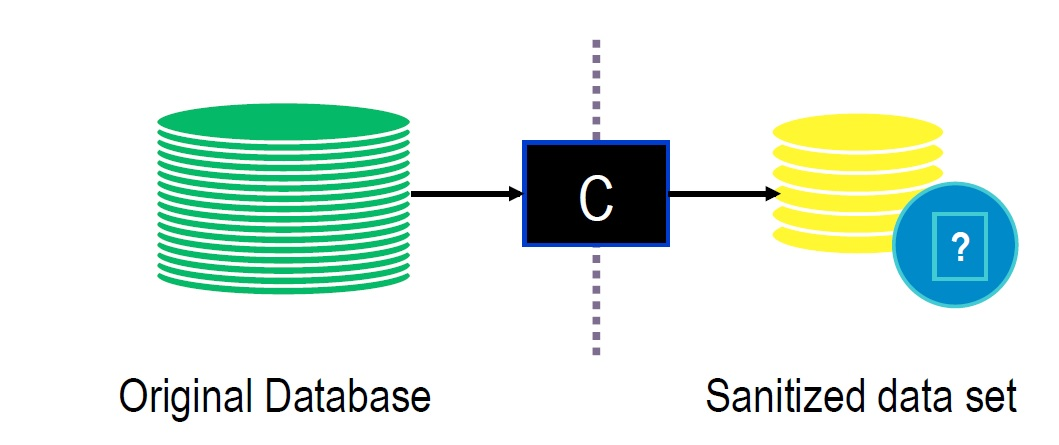
\includegraphics{privacy_dream.jpg}
    }
  }
\end{column}%
\end{columns}
\end{frame}

\begin{frame}[allowframebreaks]%
	\frametitle{Differential Privacy and Inferential Disclosure}
	Mechanism $M$ is \emph{$\varepsilon$-differentially private} if
		\begin{equation*}
		\ln\left(\frac{\Pr \left[ M(x,Q)\in B \ |x,Q\right]}{\Pr \left[
			M(x^{\prime },Q)\in B \ |x^{\prime},Q\right]}\right)
			 \leq \varepsilon 
	    \end{equation*}%
	 \footnotesize \color{darkgray} 
	 \color{black}\normalsize \\
	 \ \\
	\textbf{Properties}
	\begin{wideitemize}
	    \item \emph{Data reconstruction:} $\varepsilon$ bounds change in output from changing input
	    \item \emph{Privacy loss:} $\varepsilon$ bounds ``worst-case'' update about $x$
	    \item \emph{Composes:} Losses due to multiple uses of the same data are ``added up''
	    \item \emph{Future Proof:} Guarantees independent of outside knowledge
	    \item \emph{Public:} Mechanism and parameters can be published [\emph{SDL-aware analysis}]
	\end{wideitemize}
\end{frame}%

\begin{frame}[allowframebreaks]%
  \frametitle{Defining Accuracy}
  % We define accuracy in terms of the squared $\ell_2$ distance between the mechanism output and the exact answer $Q(x)$.
\begin{definition}[Accuracy ($I$)]
  \label{def:accuracy}
  Given histogram $x \in \mathbb{Z}^{\ast |\chi |}$ and query workload $Q \in  \mathcal{F}$, the data publication mechanism $M(x,Q)$ has accuracy $I$ if
  $$\mathbb{E}\left[\left\Vert(M(x,Q) - Q(x)\right\Vert^{2}_{2}\right] = -I.$$ where $I\le 0$ and the expectation is taken only over the randomness in $M(x,Q)$.
\end{definition}
\begin{wideitemize}
  \item $\left\Vert\cdot\right\Vert^{2}_{2}$ is the square of the $\ell_{2}$ distance.
  \item expectations taken over the distn.\ induced by $M(x,Q)$.
\end{wideitemize}
%In this definition, .

\end{frame}%

\begin{frame}[allowframebreaks]%
  \frametitle{Differential Privacy as Production Technology}
  We argue that some DP mechanisms are proper production technologies: $X$-efficient for accuracy, given privacy loss
\vskip.25in
  {\Large\textbf{Examples:}}
  \begin{wideitemize}
    \item \emph{Randomized Response}
    \item \emph{Laplace Mechanism}
    \item \emph{Matrix Mechanism}
  \end{wideitemize}
\end{frame}%

\begin{frame}[allowframebreaks]%
  \frametitle{Laplace Mechanism}
  \begin{theorem}[Laplace Mechanism]
  \label{prop:laplace_mechanism}
   For $\varepsilon>0$, query workload $Q$, and histogram $x$, define data publication mechanism
   $\limfunc{Lap}(x,Q) \equiv Qx + e$,
   where $e$ is a conformable vector of iid samples drawn from the Laplace distribution with scale parameter
   $b=\frac{\Delta Q }{\varepsilon}$.
   $Lap(x,Q)$ is $\varepsilon$-differentially private.
\end{theorem}
\begin{wideitemize}
  \item $\Delta Q$ is sensitivity of the query workload
  \item Data indepedent
  \item Yields a concave production relationship:
  $$ I = -\frac{2L\left(\Delta Q\right)^{2}}{\varepsilon^{2}}$$
  when $L$ is the total number of queries
\end{wideitemize}
\end{frame}%


%%%%%%%%%%%%%%%%%%%%%%%%%%%%%%%%%%%%%%%%%%%%%%%%%%%%%%%%%%%%%%%%%
%%%%%%%%%%%%%%%%%%%%%%%%%%%%%%%%%%%%%%%%%%%%%%%%%%%%%%%%%%%%%%%%%

\section{Application to Title I Funding}
\begin{transitionframe}
  \begin{center}
    \Huge Application to Title I
  \end{center}
\end{transitionframe}

\begin{frame}{Setting}
  \begin{wideitemize}
    \item Title I funds appropriated by Congress to needy school districts
    \item DOE allocates to district $\ell$ using 
$$
	A_{\ell} = E_{\ell}\times C_{\ell},
$$
    \begin{itemize}
    	\item $A_{\ell}$ is the \emph{authorization amount}
    	\item $E_{\ell}$ is the \emph{eligibility count}
    	\item $C_{\ell}$ is the \emph{adjusted per-pupil expenditure}
    \end{itemize}
    \item Census publishes $\widehat{E}_{\ell}$
    \item \textbf{Target Allocation:} $X = \sum_{\ell=1}^{L} E_{\ell}\times C_{\ell}$
    \item \textbf{Actual Allocation:} $\widehat{X} = \sum_{\ell=1}^{L} \widehat{E}_{\ell}\times C_{\ell}$
  \end{wideitemize}
  {\textbf{Policy challenge:} balance privacy loss among disadvantaged households against misallocation of Title I funds}
\end{frame}

\begin{frame}{Publication Mechanism}
  \begin{wideitemize}
  	\item \textbf{Database:} Households with indicator for Title I eligibility and district geocode
  	\item \textbf{Queries:} Count of Title I households by district ($E_{\ell}$)
  	\item \textbf{Mechanism:} Laplace Mechanism (Matrix Mechanism)
  	\begin{itemize}
  		\item Publish $\widehat{E}_{\ell} = E_{\ell}+e_{\ell}$ 
  		\item $e_{\ell}$ is Laplace noise with scale parameter $\varepsilon^{-1}$
  		\item Satisfies $\varepsilon-$differential privacy
  		\item Accuracy:
			$$
				I = -\mathbb{E}\left[\sum_{\ell=1}^{L}\left(\widehat{E}_{\ell}-E_{\ell}\right)^{2}\right] = -\frac{2L}{\varepsilon^{2}}
			$$
  	\end{itemize}
  \end{wideitemize}
\end{frame}

\begin{frame}{Social Welfare Function}
\begin{equation*}
  SWF = \phi\sum_{i}v_{i}^{Info}(\varepsilon) + (1-\phi)v^{Data}(I),
\end{equation*}
  \begin{wideitemize}
    \item Weight, $0\le\phi\le1$, on privacy preferences
    \item \textbf{Information Utility:} $v_{i}^{Info}(\varepsilon) = -k_{i}\varepsilon$
    \item \textbf{Data Utility:} $v^{Data}(I) = a_{i} + b_{i} I$

  \end{wideitemize}
\end{frame}



%%%%%%%%%%%%%%%%%%%%%%%%%%%%%%%%%%%%%%%%%%%%%%%%%
%Preferences for privacy
\begin{transitionframe}
  \begin{center}
    \Huge Information Utility
  \end{center}
\end{transitionframe}

\begin{frame}{Information Utility}
  (based on Ghosh and Roth [2015])
  \begin{wideitemize}
    \item Let $\Omega$ be a set of future states that can be affected by disclosure \ \\
    e.g., identity theft; denial of health insurance; persecution
    \item Utility: $u_{i}(\omega)$ with $\omega\in\Omega$
    \item Mechanism: $M(x,Q)$ has output drawn from $\mathcal{R}$ 
    \item $M(x,Q)$ is $\varepsilon$-differentially private
  \end{wideitemize}

\end{frame}

\begin{frame}{Information Utility}
  \begin{wideitemize}
    \item Let $z:\mathcal{R}\rightarrow\Delta\Omega$ map mechanism output to probabilities of future states
    \item Question: How much worse off is $i$ when her data is included in $x$ versus when it is excluded?
    \item Claim: Mechanism $Z(x,Q) = z(M(x,Q))$ is $\varepsilon$-differentially private 
    \item Let $x^\prime$ be a neighboring database that excludes $i$'s data   
  \end{wideitemize}
  It follows that
$$\mathbb{E}_{\omega|M(x,Q)}\left[u_{i}(\omega)\right] \le e^{\varepsilon}\mathbb{E}_{\omega|M(x^\prime,Q)}\left[u_{i}(\omega)\right]$$
  Worst case incremental utility change is:
  $$\Delta U = \left(e^{\varepsilon}-1\right)k_{i}$$ 
  $k_{i}$ is expected utility over future events when $i$'s data are \emph{not} included in the mechanism.\ \\
  When $\varepsilon \approx 0$
  $$\left(e^{\varepsilon}-1\right)k_{i}\approx\varepsilon k_{i}$$
\end{frame}

%%%%%%%%%%%%%%%%%%%%%%%%%%%%%%%%%%%%%%%%%%%%%%%%%
%Preferences for privacy
\begin{transitionframe}
  \begin{center}
    \Huge Data Utility
  \end{center}
\end{transitionframe}

\begin{frame}{Data Utility}
  \textbf{Result:} reduced-form linear in accuracy: $v^{data}_{i}(I) =  a_{i} + b_{i}I$
  \begin{wideitemize}
    \item utility from wealth: $U_{i}(W_{i})$ (strictly concave)
    \item $W_{i} = \Pi_{i}^{T} M(x,Q)$ 
    \begin{itemize}
      \item $M(x,Q) = Qx + e$ is Laplace mechanism
      \item $\Pi_{i}$ is a vector of weights
    \end{itemize} 
  \end{wideitemize}

  
\end{frame}

\begin{frame}{Data Utility}
 Expected utility for any person $i$ is
$$
  \mathbb{E}\left[U_{i}(W_{i})\right] = \mathbb{E}_{x}\left[\mathbb{E}_{e|x}\left[U_{i}\left(\Pi_{i}^{T}Qx + \Pi_{i}^{T}e\right)\vert x\right] \right].
$$
approximated as
 \begin{equation}
  \begin{array}{rcl}
   \mathbb{E}\left[U_{i}(W_{i})\right]  \approx &  \mathbb{E}_{x}\left[U_{i}(\Pi_{i}^{T}Qx)\right] &- I\cdot \left\{\frac{1}{2}\mathbb{E}_{x}\left[U_{i}^{\prime\prime}(\Pi_{i}^{T}Qx)\right] \frac{\left\Vert \Pi_{i}^{T} \right\Vert^{2}}{L}\right\} \\
   \equiv & a_{i} & + I\cdot b_{i}.
   \end{array}
 \end{equation}
 \end{frame}
  
%%%%%%%%%%%%%%%%%%%%%%%%%%%%%%%%%%%%%%%%%%%%%%%%%
%Preferences for privacy
\begin{transitionframe}
  \begin{center}
    \Huge Back to the Title I Application
  \end{center}
\end{transitionframe}

\begin{frame}{Social Welfare Function}
\begin{equation*}
  SWF = \phi\sum_{i}v_{i}^{Info}(\varepsilon) + (1-\phi)v^{Data}(I),
\end{equation*}
  \begin{wideitemize}
    \item Weight, $0\le\phi\le1$, on privacy preferences
    \item \textbf{Information Utility:} $v_{i}^{Info}(\varepsilon) = -k_{i}\varepsilon$ %[\citet{Ghosh:Auction:GEB:2015}]
    \item \textbf{Data Utility:} $v^{Data}(I)$
      \begin{itemize}
        \item Linear-quadratic in aggregate misallocation: $W=(\widehat{X}-X) = \sum_{\ell=1}^{L}C_{\ell}\left[\widehat{E}_{\ell}-E_{\ell}\right]$
        \item $v^{Data}(I)=I\sum_{\ell=1}^{L}\frac{C_{\ell}^{2}}{L}$
      \end{itemize}
  \end{wideitemize}
\end{frame}


\begin{frame}{Calibration}
\begin{columns}[T] % align columns
\begin{column}{.58\textwidth}
		\begin{equation*}
			WTA \equiv \frac{dI}{d\varepsilon} = \left(\frac{\phi}{1-\phi}\right) N\frac{\bar{k}}{\bar{C^{2}}},
		\end{equation*}
  \begin{wideitemize}
    \item $L=13,000$ public school districts
    \item $N=46$ million school-age children
    \item average squared spending, $\bar{C^{2}}\approx 20$ million
    \item $\bar{k}=\$1,400$ (avg.\ cost of identity theft)
    \item Setting $WTA = MRT$ 
      $$\varepsilon = 2.52\times \left(\frac{\phi}{1-\phi}\right)^{-\frac{1}{3}}$$
  \end{wideitemize}
\end{column}%
\hfill%
\begin{column}{.38\textwidth}
  \makebox[\linewidth][c]{
    \resizebox{\linewidth}{!}{
      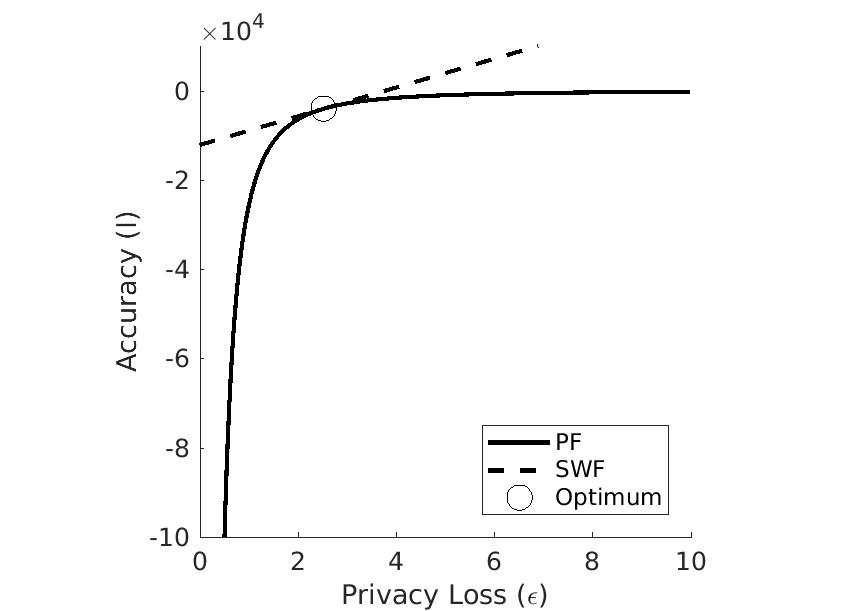
\includegraphics{plannersprob.jpg}
    }
  }
\end{column}%
\end{columns}
\end{frame}

\begin{frame}[fragile]{Calibration}
\begin{columns}[T] % align columns
\begin{column}{.58\textwidth}
  $$\eta = \frac{\phi}{1-\phi}$$
  \begin{wideitemize}
    \item<1-> $\eta=1$
    \begin{itemize}
    	\item<2->  $\varepsilon^{\ast}=2.52$
    	\item<2->  $RMSE:$ \$2,509 (70 cents per student)
    \end{itemize}
    \item<3-> $\eta= \frac{N}{POP-N}\approx 0.15$
    \begin{itemize}
    	\item<4-> $\varepsilon^{\ast\ast} = 4.74$
    	\item<4-> $RMSE:$ \$1,334 (38 cents per student)
    \end{itemize}
    \item<5-> Privacy advocates urge $\varepsilon<<1$
    \begin{itemize}
    	\item<6-> Fix $\varepsilon=0.1$
    	\item<6-> $RMSE: $\$63,000 (\$18 per student)
    \end{itemize}
  \end{wideitemize}
\end{column}%
\hfill%
\begin{column}{.38\textwidth}
  \makebox[\linewidth][c]{
    \resizebox{\linewidth}{!}{
      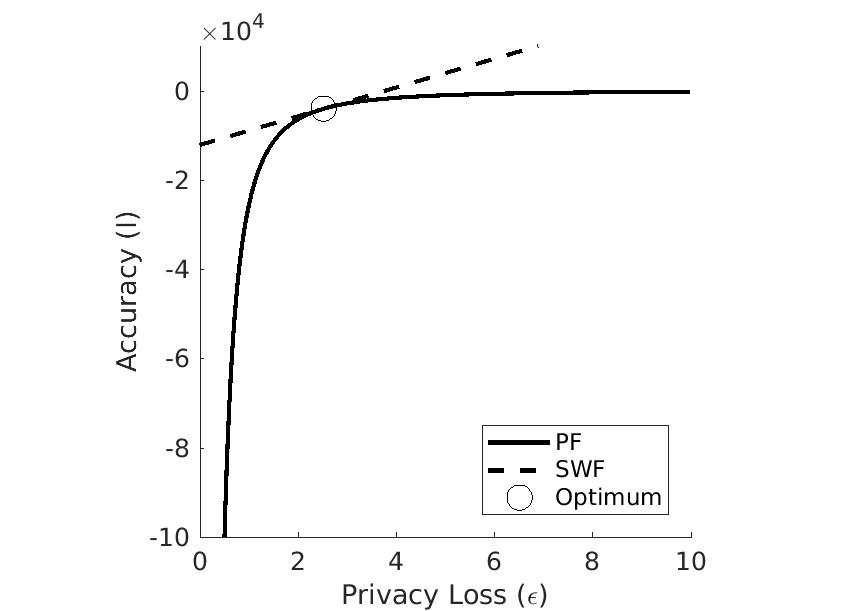
\includegraphics{plannersprob.jpg}
    }
  }
\end{column}%
\end{columns}
\end{frame}

%%%%%%%%%%%%%%%%%%%%%%%%%%%%%%%%%%%%%%%%%%%%%%%%%
%Other applications
\begin{transitionframe}
  \begin{center}
    \Huge Other Applications
  \end{center}
\end{transitionframe}

\begin{frame}{Legislative Redistricting}
  \begin{wideitemize}
    \item Data utility is based on
    \begin{itemize}
        \item Supreme Court one-person one-vote decision (all legislative districts must have approximately equal populations; there is judicially approved variation)
        \item Statistical disclosure limitation is a “statistical method” (permitted by Utah v. Evans) not “sampling” (prohibited by the Census Act, confirmed in Commerce v. House of Representatives)
        \item Voting Rights Act, Section 2: requires majority-minority districts at all levels, when certain criteria are met
    \end{itemize}
    \item The privacy utility is based on
    \begin{itemize}
        \item Title 13 requirement not to publish exact identifying information
        \item The public policy implications of uses of race, ethnicity and citizenship tabulations at detailed geography
    \end{itemize}
  \end{wideitemize}
\end{frame}

\begin{frame}{Economic Censuses and National Accounts}
  \begin{wideitemize}
    \item The major client is the producer of national accounts
    \item In most countries these activities are consolidated in a single agency
    \item Data utility: accuracy of the national accounts
    \item Privacy utility: sensitivity of detailed industry and product data
    \item Detailed tables can be produced using formal privacy with far less suppression bias than in current methods
    \item But it's an inefficient use of the global privacy-loss budget when the accounts are published at much more aggregated levels
    \item Optimize the data and privacy utility trade-offs by sharing confidential data (as permitted under CIPSEA) and applying formal privacy at publication level
  \end{wideitemize}
\end{frame}

\begin{frame}{Tax Data and Tax Simulations}
  \begin{wideitemize}
    \item Simulating the effects of tax policy changes is an important use of tax micro-data
    \item Traditional disclosure limitation methods aggravate these simulations by smoothing over important kinks and breaking audit consistency
    \item Data utility: quality of the simulated tax policy effects
    \item Privacy utility: sensitivity of the income tax returns
    \item Detailed tables can be produced using formal privacy with far less suppression bias than in current methods
    \item But it's an inefficient use of the global privacy-loss budget when the accounts are published at much more aggregated levels
    \item Optimize the data and privacy utility trade-offs by doing the simulations inside the IRS firewall and applying formal privacy protection to outputs
  \end{wideitemize}
\end{frame}

\begin{frame}{General Purpose Public-use Micro-data}
  \begin{wideitemize}
    \item Hierarchy of users
    \begin{itemize}
        \item Educational
        \item Commercial
        \item Scientific
    \end{itemize}
    \item Data utility: valid scientific inferences on arbitrary hypotheses estimable within the design of the confidential data product 
    \item Privacy utility: reconstruction-abetted re-identification attacks make every variable a potential identifier, especially in combination
    \item Traditional SDL fails the data utility condition
    \item Formal privacy guarantees the data utility for hypotheses in the query workload--serves educational and commercial users well
    \item Other scientific hypotheses may require restricted-access to the micro-data and specialized analysis software
  \end{wideitemize}
\end{frame}

\begin{transitionframe}
  \begin{center}
    \Huge Thank  you
  \end{center}
    \begin{center}
    John.Maron.Abowd@census.gov
  \end{center}

\end{transitionframe}
%%%%%%%%%%%%%%%%%%%%%%%%%%%%%%%%%%%%%%%%%%%%%%%%%%%%%%%%%%%%%%%%%
%%%%%%%%%%%%%%%%%%%%%%%%%%%%%%%%%%%%%%%%%%%%%%%%%%%%%%%%%%%%%%%%%



%%%%%%%%%%%%%%%%%%%%%%%%%%%%%%%%%%%%%%%%%%%%%%%%%%%%%%%%%%%%%%%%%
%%%%%%%%%%%%%%%%%%%%%%%%%%%%%%%%%%%%%%%%%%%%%%%%%%%%%%%%%%%%%%%%%

\appendix

\begin{transitionframe}
  \begin{center}
    \Huge Appendix Slides
  \end{center}
\end{transitionframe}

\section{Data Publication Model}
\begin{transitionframe}
  \begin{center}
    \Huge Data Publication Model
  \end{center}
\end{transitionframe}



\begin{frame}{Database}
\begin{columns}[T] % align columns
\begin{column}{.58\textwidth}
  \begin{wideitemize}
	  \item Custodian holds a database matrix, $D$
	  \item Rows of $D$ are for $N$ individuals
	  \item Columns record variables / features.
	  \item Each column is drawn from a finite-valued \emph{data domain}, $\chi$
  \end{wideitemize}

  % {\Large Histogram Representation}
  
  % \begin{wideitemize}
	 %  \item The \emph{histogram representation} of $D$, $x \in  \mathbb{Z}^{\ast |\chi |}$
	 %  \item For each $k\in\chi$, $x_{k}$ is the number of records in $D$ with attribute combination $k$.
  % \end{wideitemize}
\end{column}%
\hfill%
\begin{column}{.38\textwidth}
  \makebox[\linewidth][c]{
    \resizebox{\linewidth}{!}{
      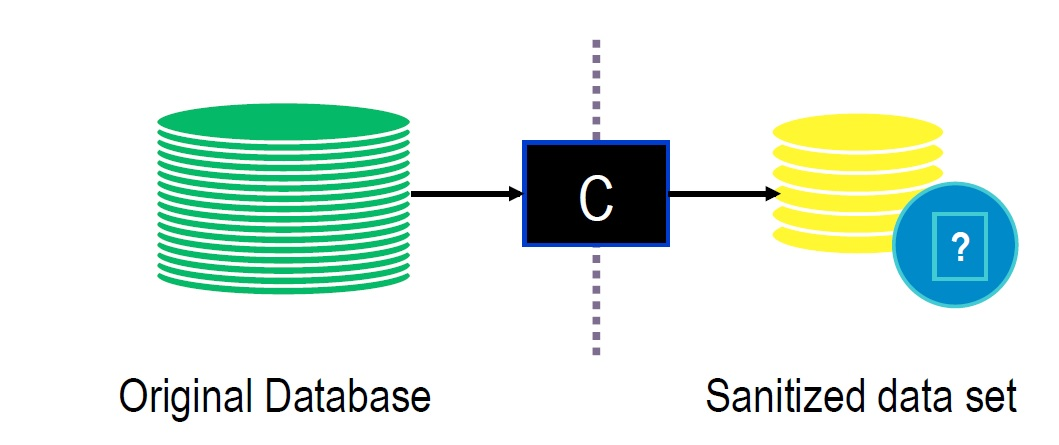
\includegraphics{privacy_dream.jpg}
    }
  }
\end{column}%
\end{columns}
\end{frame}

\begin{frame}{Queries}
\begin{columns}[T] % align columns
\begin{column}{.58\textwidth}
  \begin{wideitemize}
	  \item \emph{database query} is $q:\mathbb{Z}^{\ast |\chi |}\rightarrow \mathcal{R}$
	  \item $q(x)$ is the \emph{exact query answer}
	  \item \emph{query workload}, $Q=\{q_{1},\ldots,q_{k} \}$.
	  \item The $\ell_{1}$ sensitivity for query $q$ 
		\begin{definition}[$\ell_{1}$ Query Sensitivity]
			\label{def:query_sensitivity}
			\begin{equation*}
				\Delta q = \max_{x,y\in \mathbb{Z}^{\ast |\chi |}, \left\Vert{x}-{y}\right\Vert_{1} \le 1}|q(x)-q(y)|.
			\end{equation*}
		\end{definition}
  \end{wideitemize}
\end{column}%
\hfill%
\begin{column}{.38\textwidth}
  \makebox[\linewidth][c]{
    \resizebox{\linewidth}{!}{
      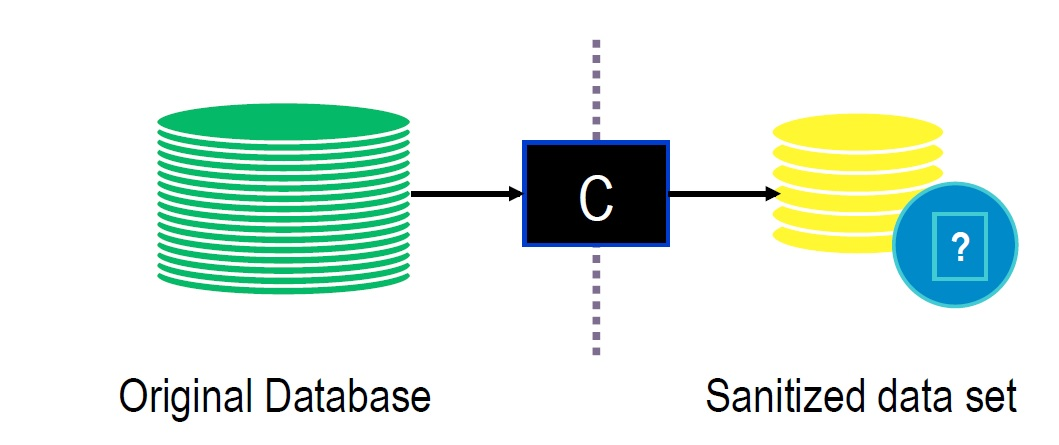
\includegraphics{privacy_dream.jpg}
    }
  }
\end{column}%
\end{columns}
\end{frame}

\begin{frame}{Data Publication Mechanism}
\begin{columns}[T] % align columns
\begin{column}{.58\textwidth}
	\begin{definition}[Data Publication Mechanism]
	\label{def:query_mechanism} Let $\mathcal{F}$ be the set of allowable query workloads.
	A \emph{data publication mechanism} is a random function
	$M:\mathbb{Z}^{\ast |\chi|}\times \mathcal{F}\rightarrow \mathcal{R}$ whose
	inputs are a histogram $x\in \mathbb{Z}^{\ast |\chi |}$ and a workload $Q \in  \mathcal{F}$,
	and whose random output is an element of range $\mathcal{R}$.
	For  $B \in \mathcal{B}$, where $\mathcal{B}$ are the measurable subsets of $\mathcal{R}$,
	the conditional probability is $\Pr \left[ M(x,Q)\in B | x,Q \right] $, given $x$ and $Q$, where
	the probabilities are over the randomness induced by the mechanism.
	\end{definition}
\end{column}%
\hfill%
\begin{column}{.38\textwidth}
  \makebox[\linewidth][c]{
    \resizebox{\linewidth}{!}{
      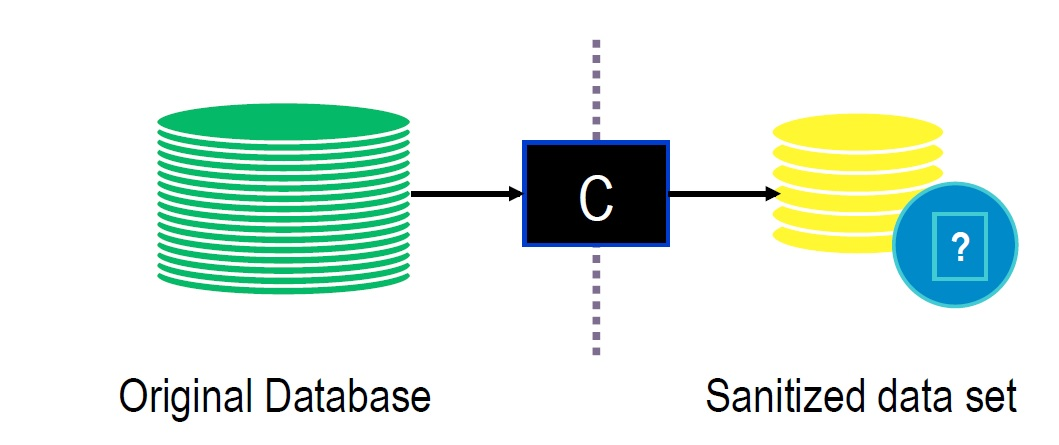
\includegraphics{privacy_dream.jpg}
    }
  }
\end{column}%
\end{columns}
\end{frame}

\section{Production}
\begin{transitionframe}
  \begin{center}
    \Huge Production Possibilities
  \end{center}
\end{transitionframe}

\begin{frame}{Defining Production}
\begin{columns}[T] % align columns
\begin{column}{.58\textwidth}
  \begin{wideitemize}
    \item Differential privacy, $\varepsilon$
    \item Data accuracy, $I$
    \item Transformation sets
  \end{wideitemize}
\end{column}%
\hfill%
\begin{column}{.38\textwidth}
  \makebox[\linewidth][c]{
    \resizebox{\linewidth}{!}{
      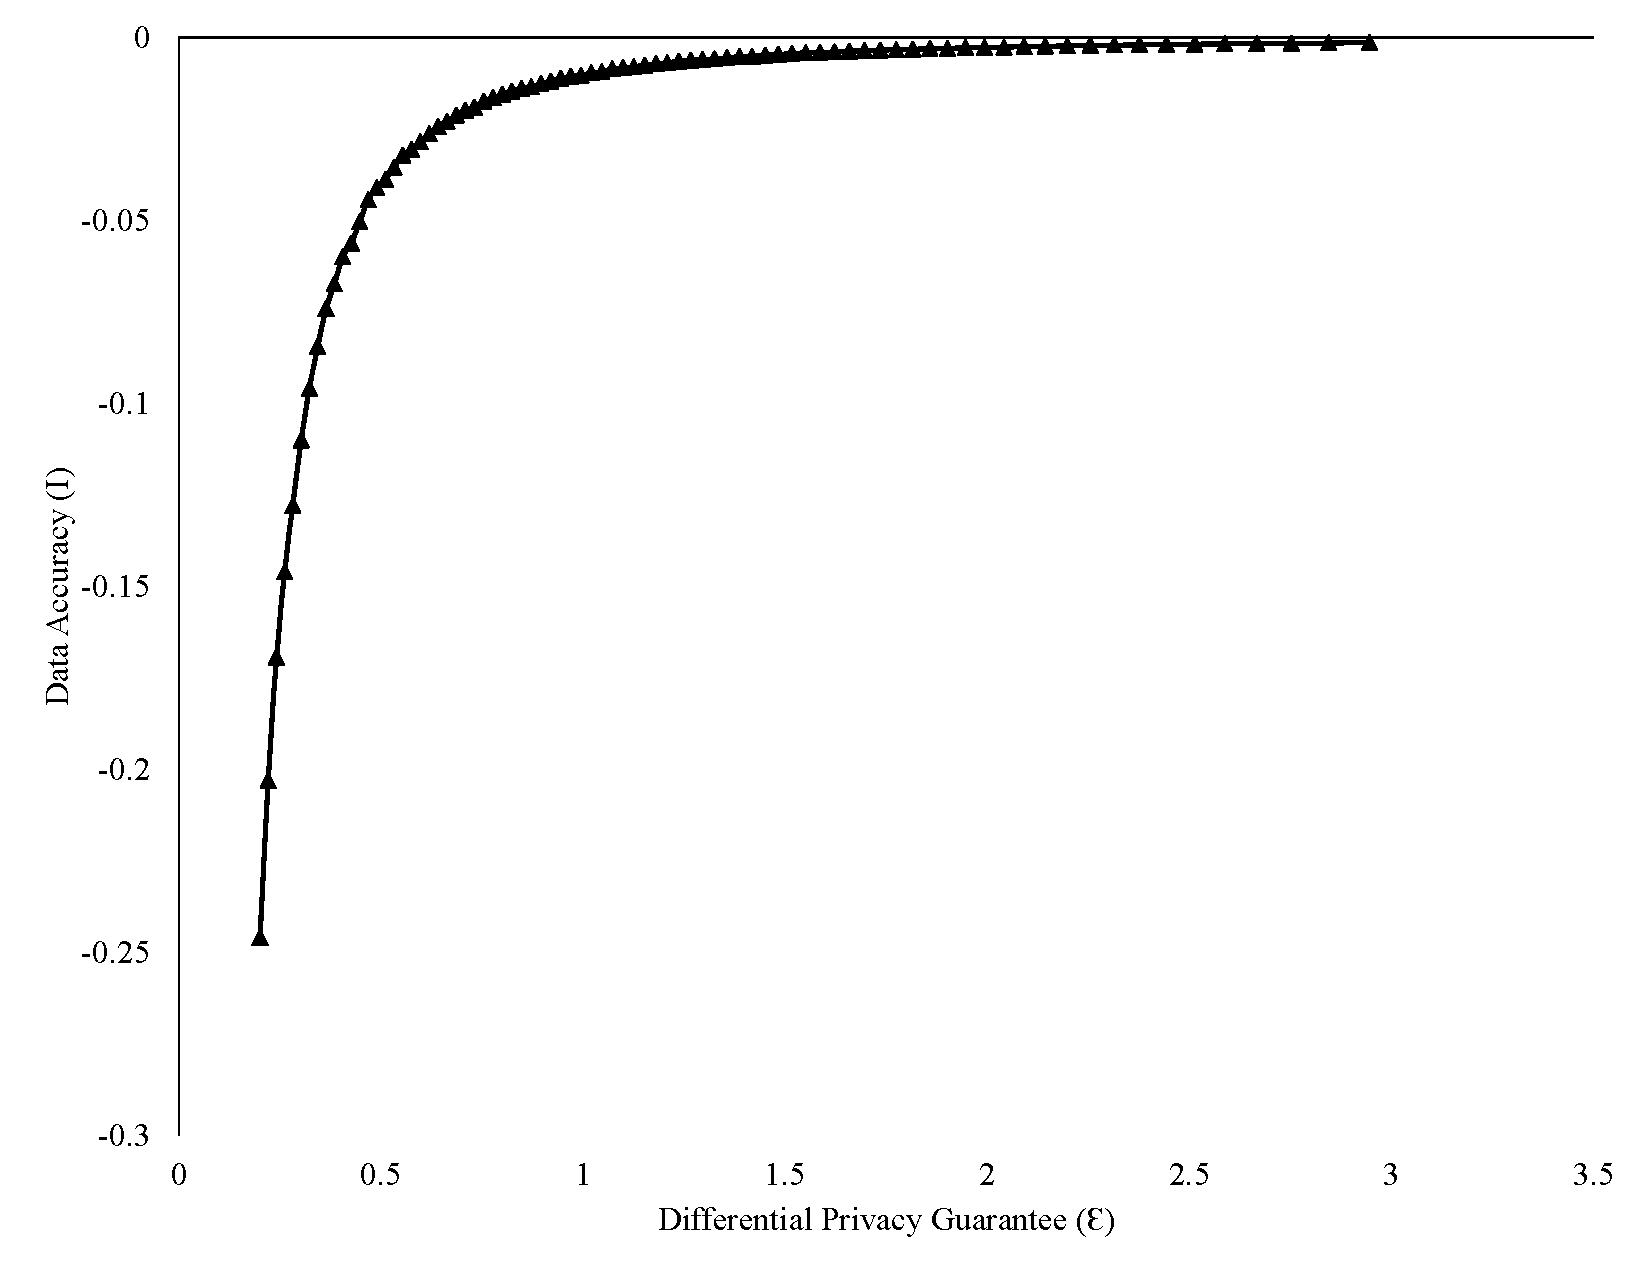
\includegraphics{RandResponse_Plot.pdf}
    }
  }
\end{column}%
\end{columns}
\end{frame}

\begin{frame}{Differential Privacy}
\begin{columns}[T] % align columns
\begin{column}{.58\textwidth}
Mechanism $M$ is \emph{$\varepsilon$-differentially private} if
	\begin{wideitemize}
		\item For all neighboring $x,x^{\prime}$, $Q$, and $B$
		\begin{equation*}
		\ln\left(\frac{\Pr \left[ M(x,Q)\in B \ |x,Q\right]}{\Pr \left[
			M(x^{\prime },Q)\in B \ |x^{\prime},Q\right]}\right)
			 \leq \varepsilon 
	    \end{equation*}%
	\end{wideitemize}
\end{column}%
\hfill%
\begin{column}{.38\textwidth}
  \makebox[\linewidth][c]{
    \resizebox{\linewidth}{!}{
      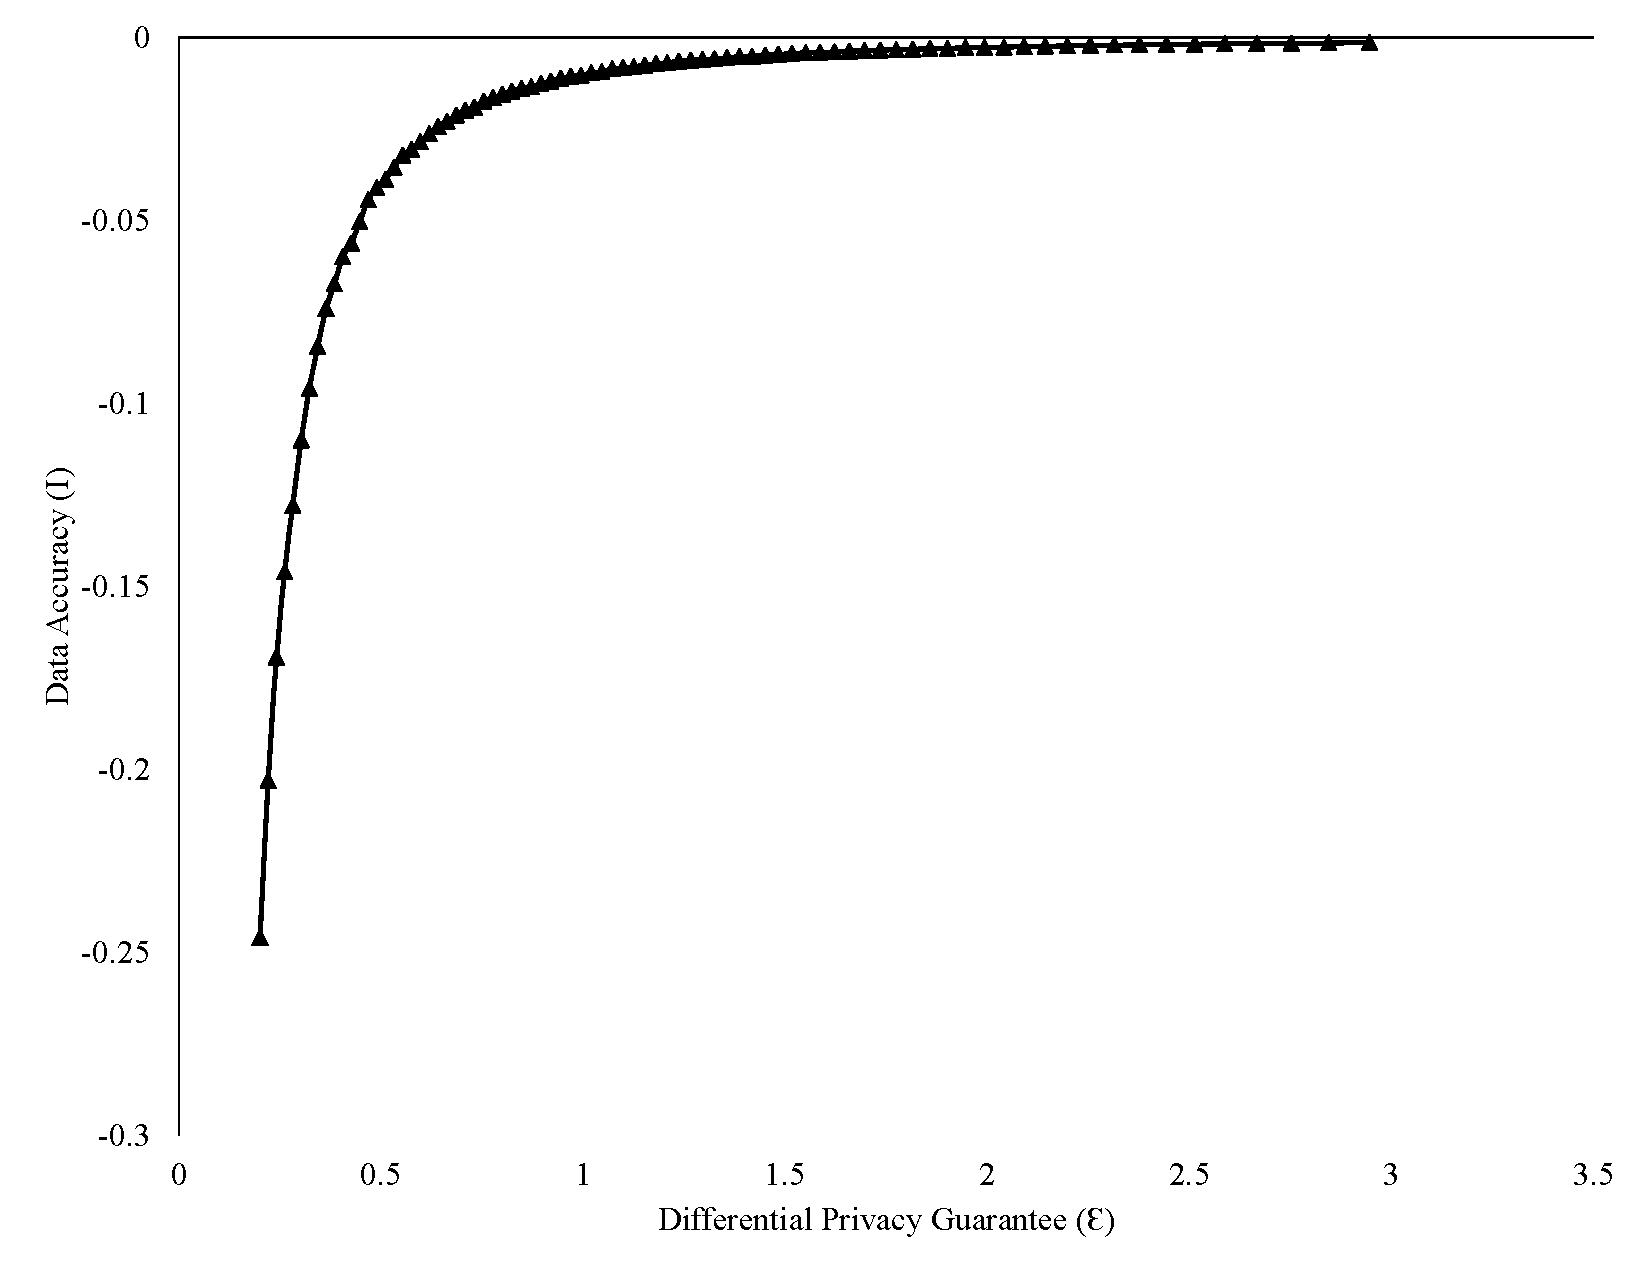
\includegraphics{RandResponse_Plot.pdf}
    }
  }
\end{column}%
\end{columns}
\end{frame}

\begin{frame}{Data Accuracy}
\begin{columns}[T] % align columns
\begin{column}{.58\textwidth}
	\begin{wideitemize}
	    \item Mechanism $M$ has accuracy $I<0$ if
	     $$\mathbb{E}\left[\left\Vert(M(x,Q) - Q(x)\right\Vert^{2}_{2}\right] = -I.$$
	     \item $\left\Vert\cdot\right\Vert^{2}_{2}$ is the square of the $\ell_{2}$ (Euclidean) distance.
	\end{wideitemize}

\end{column}%
\hfill%
\begin{column}{.38\textwidth}
  \makebox[\linewidth][c]{
    \resizebox{\linewidth}{!}{
      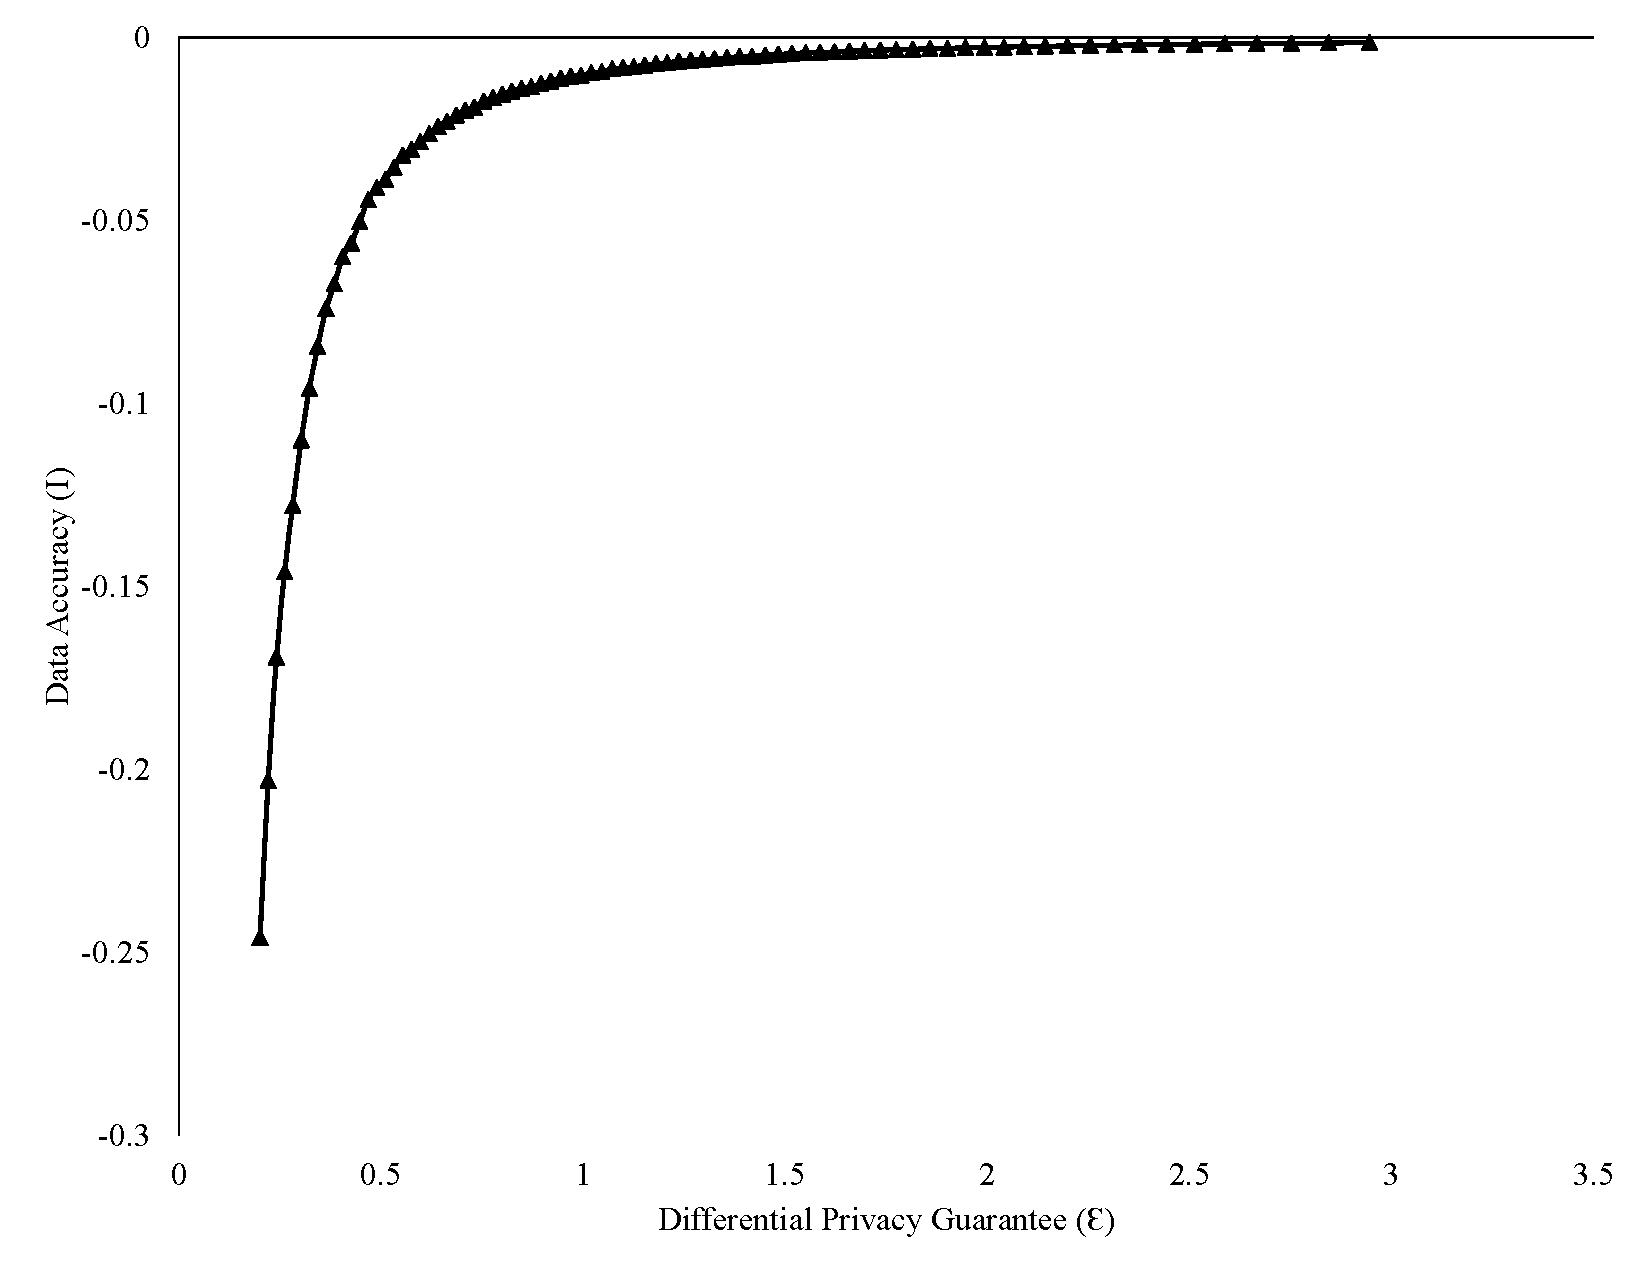
\includegraphics{RandResponse_Plot.pdf}
    }
  }
\end{column}%
\end{columns}
\end{frame}

\begin{frame}[allowframebreaks]{Transformation Sets}
\begin{columns}[T] % align columns
\begin{column}{.58\textwidth}
	\begin{wideitemize}
	    \item Each mechanism, $M$, has associated \emph{production activity} $(\varepsilon,I)$
	    \item Custodian's \emph{transformation set},
	    $$Y=\left\{ \left( \varepsilon ,I \right) \left\vert \varepsilon >0,I<0 \right. \right\}$$
	    \item \textbf{Assumptions}
	    \begin{itemize}
	    	\item $Y$ is closed and bounded
	    	\item no free lunch [\citet{Dwork2004}, \citet{Dwork2008}, \citet{gehrke2011towards}, \citet{Kifer:2011:NFL:1989323.1989345}]
	    \end{itemize}
	 %    \item \emph{transformation function} $G(\varepsilon,I)$
		% $
		% Y=\left\{ \left( \varepsilon ,I \right) \left\vert \varepsilon >0,I<0 \text{ s.t. }G(\varepsilon ,I)\leq0
		% \right\}\right\}.
		% $
		\item The \emph{production frontier}
		$$
		PF=\left\{ \left( \varepsilon ,I\right)
		\left\vert \varepsilon >0,I<0\text{ s.t. }G(\varepsilon ,I)=0\right.
		\right\}
		$$
	\end{wideitemize}
\end{column}%
\hfill%
\begin{column}{.38\textwidth}
  \makebox[\linewidth][c]{
    \resizebox{\linewidth}{!}{
      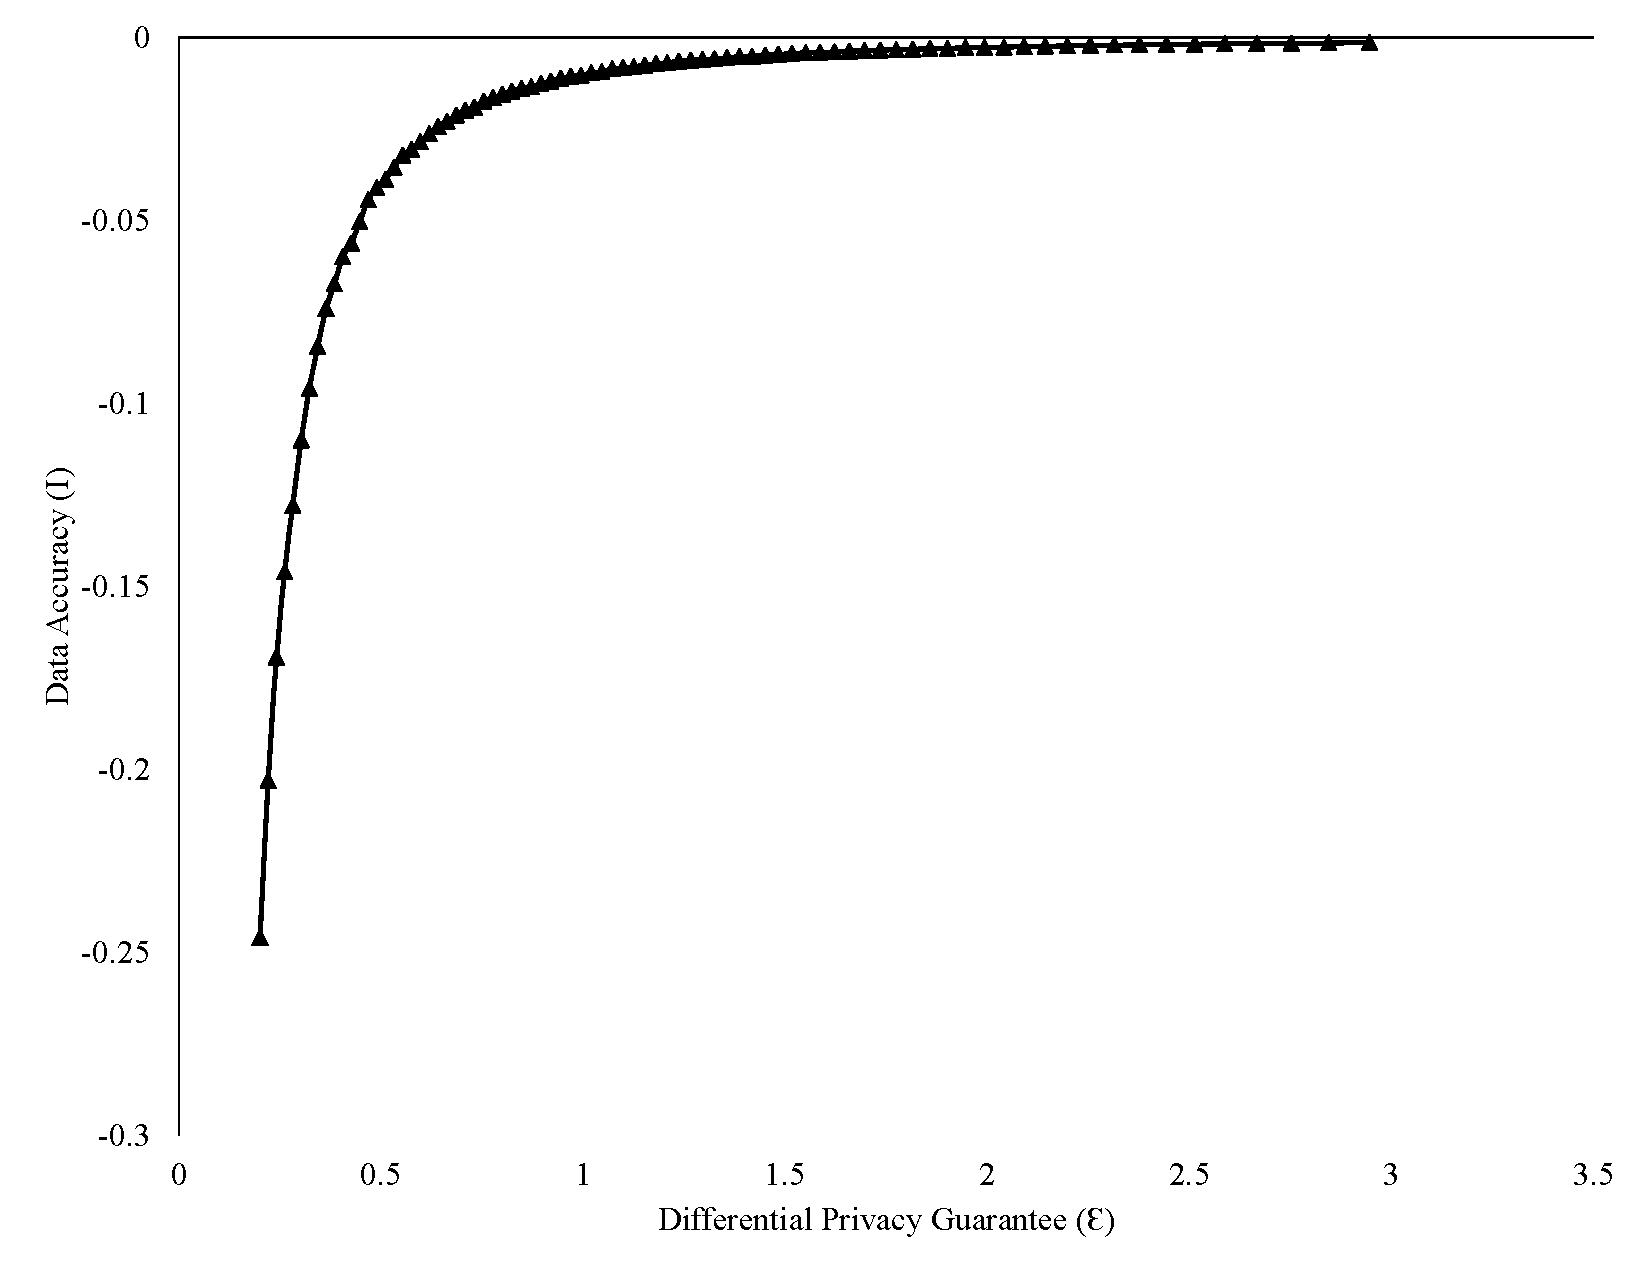
\includegraphics{RandResponse_Plot.pdf}
    }
  }
\end{column}%
\end{columns}
\end{frame}


%%%%%%%%%%%%%%%%%%%%%%%%%%%%%%%%%%%%%%%%%%%%%%%%%%%%%%%%%%%%%%%%%
%%%%%%%%%%%%%%%%%%%%%%%%%%%%%%%%%%%%%%%%%%%%%%%%%%%%%%%%%%%%%%%%%


%\section[References]{References}

%\begin{frame}[allowframebreaks]

%\frametitle{References}
%\def\newblock{\hskip .11em plus .33em minus .07em} % important line
%\bibliographystyle{dcu}
%\bibliography{library}
%\end{frame}%

\end{document}


